\documentclass[a4paper, 12pt]{book}
%\documentclass[a4paper, 12pt, draft]{book}  Nalogo preverite tudi z opcijo draft, ki vam bo pokazala, katere vrstice so predolge!

\usepackage[utf8x]{inputenc}   % omogoča uporabo slovenskih črk kodiranih v formatu UTF-8
\usepackage[slovene,english]{babel}    % naloži, med drugim, slovenske delilne vzorce
\usepackage[pdftex]{graphicx}  % omogoča vlaganje slik različnih formatov
\usepackage{fancyhdr}          % poskrbi, na primer, za glave strani
\usepackage{amssymb}           % dodatni simboli
\usepackage{amsmath}           % eqref, npr.
%\usepackage{hyperxmp}
\usepackage[hyphens]{url}  % dodal Solina
\usepackage{comment}       % dodal Solina

\usepackage[pdftex, colorlinks=true,
						citecolor=black, filecolor=black, 
						linkcolor=black, urlcolor=black,
						pagebackref=false, 
						pdfproducer={LaTeX}, pdfcreator={LaTeX}, hidelinks]{hyperref}

\usepackage{color}       % dodal Solina
\usepackage{soul}       % dodal Solina

\usepackage{longtable}  % dodal jaz
\usepackage{minted}      % dodal jaz
\usemintedstyle{bw}    % dodal jaz

%%%%%%%%%%%%%%%%%%%%%%%%%%%%%%%%%%%%%%%%
%	DIPLOMA INFO
%%%%%%%%%%%%%%%%%%%%%%%%%%%%%%%%%%%%%%%%
\newcommand{\ttitle}{Visoko skalabilna NewSQL relacijska podatkovna baza CockroachDB}
\newcommand{\ttitleEn}{Higly scalable NewSQL relational database CockroachDB}
\newcommand{\tsubject}{\ttitle}
\newcommand{\tsubjectEn}{\ttitleEn}
\newcommand{\tauthor}{Matjaž Mav}
\newcommand{\tkeywords}{podatkovne baze, skaliranje, SQL, NewSQL, CockroachDB, PostgreSQL, Citus, YCSB}
\newcommand{\tkeywordsEn}{databases, scalability, SQL, NewSQL, PostgreSQL, Citus, YCSB}


%%%%%%%%%%%%%%%%%%%%%%%%%%%%%%%%%%%%%%%%
%	HYPERREF SETUP
%%%%%%%%%%%%%%%%%%%%%%%%%%%%%%%%%%%%%%%%
\hypersetup{pdftitle={\ttitle}}
\hypersetup{pdfsubject=\ttitleEn}
\hypersetup{pdfauthor={\tauthor, mm3058@student.uni-lj.si}}
\hypersetup{pdfkeywords=\tkeywordsEn}


 


%%%%%%%%%%%%%%%%%%%%%%%%%%%%%%%%%%%%%%%%
% postavitev strani
%%%%%%%%%%%%%%%%%%%%%%%%%%%%%%%%%%%%%%%%  

\addtolength{\marginparwidth}{-20pt} % robovi za tisk
\addtolength{\oddsidemargin}{40pt}
\addtolength{\evensidemargin}{-40pt}

\renewcommand{\baselinestretch}{1.3} % ustrezen razmik med vrsticami
\setlength{\headheight}{15pt}        % potreben prostor na vrhu
\renewcommand{\chaptermark}[1]%
{\markboth{\MakeUppercase{\thechapter.\ #1}}{}} \renewcommand{\sectionmark}[1]%
{\markright{\MakeUppercase{\thesection.\ #1}}} \renewcommand{\headrulewidth}{0.5pt} \renewcommand{\footrulewidth}{0pt}
\fancyhf{}
\fancyhead[LE,RO]{\sl \thepage} 
%\fancyhead[LO]{\sl \rightmark} \fancyhead[RE]{\sl \leftmark}
\fancyhead[RE]{\sc \tauthor}              % dodal Solina
\fancyhead[LO]{\sc Diplomska naloga}     % dodal Solina


\newcommand{\BibTeX}{{\sc Bib}\TeX}

%%%%%%%%%%%%%%%%%%%%%%%%%%%%%%%%%%%%%%%%
% naslovi
%%%%%%%%%%%%%%%%%%%%%%%%%%%%%%%%%%%%%%%%  


\newcommand{\autfont}{\Large}
\newcommand{\titfont}{\LARGE\bf}
\newcommand{\clearemptydoublepage}{\newpage{\pagestyle{empty}\cleardoublepage}}
\setcounter{tocdepth}{2}	      % globina kazala

%%%%%%%%%%%%%%%%%%%%%%%%%%%%%%%%%%%%%%%%
% konstrukti
%%%%%%%%%%%%%%%%%%%%%%%%%%%%%%%%%%%%%%%%  
\newtheorem{izrek}{Izrek}[chapter]
\newtheorem{trditev}{Trditev}[izrek]
\newenvironment{dokaz}{\emph{Dokaz.}\ }{\hspace{\fill}{$\Box$}}

%%%%%%%%%%%%%%%%%%%%%%%%%%%%%%%%%%%%%%%%%%%%%%%%%%%%%%%%%%%%%%%%%%%%%%%%%%%%%%%
%% PDF-A
%%%%%%%%%%%%%%%%%%%%%%%%%%%%%%%%%%%%%%%%%%%%%%%%%%%%%%%%%%%%%%%%%%%%%%%%%%%%%%%


%%%%%%%%%%%%%%%%%%%%%%%%%%%%%%%%%%%%%%%% 
% define medatata
%%%%%%%%%%%%%%%%%%%%%%%%%%%%%%%%%%%%%%%% 
\def\Title{\ttitle}
\def\Author{\tauthor, mm3058@student.uni-lj.si}
\def\Subject{\ttitleEn}
\def\Keywords{\tkeywordsEn}

%%%%%%%%%%%%%%%%%%%%%%%%%%%%%%%%%%%%%%%% 
% \convertDate converts D:20080419103507+02'00' to 2008-04-19T10:35:07+02:00
%%%%%%%%%%%%%%%%%%%%%%%%%%%%%%%%%%%%%%%% 
\def\convertDate{%
    \getYear
}

{\catcode`\D=12
 \gdef\getYear D:#1#2#3#4{\edef\xYear{#1#2#3#4}\getMonth}
}
\def\getMonth#1#2{\edef\xMonth{#1#2}\getDay}
\def\getDay#1#2{\edef\xDay{#1#2}\getHour}
\def\getHour#1#2{\edef\xHour{#1#2}\getMin}
\def\getMin#1#2{\edef\xMin{#1#2}\getSec}
\def\getSec#1#2{\edef\xSec{#1#2}\getTZh}
\def\getTZh +#1#2{\edef\xTZh{#1#2}\getTZm}
\def\getTZm '#1#2'{%
    \edef\xTZm{#1#2}%
    \edef\convDate{\xYear-\xMonth-\xDay T\xHour:\xMin:\xSec+\xTZh:\xTZm}%
}

\expandafter\convertDate\pdfcreationdate 

%%%%%%%%%%%%%%%%%%%%%%%%%%%%%%%%%%%%%%%%
% get pdftex version string
%%%%%%%%%%%%%%%%%%%%%%%%%%%%%%%%%%%%%%%% 
\newcount\countA
\countA=\pdftexversion
\advance \countA by -100
\def\pdftexVersionStr{pdfTeX-1.\the\countA.\pdftexrevision}


%%%%%%%%%%%%%%%%%%%%%%%%%%%%%%%%%%%%%%%%
% XMP data
%%%%%%%%%%%%%%%%%%%%%%%%%%%%%%%%%%%%%%%%  
\usepackage{xmpincl}
\includexmp{pdfa-1b}

%%%%%%%%%%%%%%%%%%%%%%%%%%%%%%%%%%%%%%%%
% pdfInfo
%%%%%%%%%%%%%%%%%%%%%%%%%%%%%%%%%%%%%%%%  
\pdfinfo{%
    /Title    (\ttitle)
    /Author   (\tauthor)
    /Subject  (\ttitleEn)
    /Keywords (\tkeywordsEn)
    /ModDate  (\pdfcreationdate)
    /Trapped  /False
}


%%%%%%%%%%%%%%%%%%%%%%%%%%%%%%%%%%%%%%%%%%%%%%%%%%%%%%%%%%%%%%%%%%%%%%%%%%%%%%%
%%%%%%%%%%%%%%%%%%%%%%%%%%%%%%%%%%%%%%%%%%%%%%%%%%%%%%%%%%%%%%%%%%%%%%%%%%%%%%%

\begin{document}
\selectlanguage{slovene}
\frontmatter
\setcounter{page}{1} %
\renewcommand{\thepage}{}       % preprecimo težave s številkami strani v kazalu
\newcommand{\sn}[1]{"`#1"'}                    % dodal Solina (slovenski narekovaji)

%%%%%%%%%%%%%%%%%%%%%%%%%%%%%%%%%%%%%%%%
%naslovnica
 \thispagestyle{empty}%
   \begin{center}
    {\large\sc Univerza v Ljubljani\\%
      Fakulteta za računalništvo in informatiko}%
    \vskip 10em%
    {\autfont \tauthor\par}%
    {\titfont \ttitle \par}%
    {\vskip 3em \textsc{DIPLOMSKO DELO\\[5mm]
    UNIVERZITETNI  ŠTUDIJSKI PROGRAM\\ PRVE STOPNJE\\ RAČUNALNIŠTVO IN INFORMATIKA}\par}
    \vfill\null%
    {\large \textsc{Mentor}: izr.\ prof.\ dr.\ Matjaž Kukar\par}%
    {\vskip 2em \large Ljubljana, 2018 \par}%
\end{center}
% prazna stran
%\clearemptydoublepage      % dodal Solina (izjava o licencah itd. se izpiše na hrbtni strani naslovnice)

%%%%%%%%%%%%%%%%%%%%%%%%%%%%%%%%%%%%%%%%
%copyright stran
\thispagestyle{empty}
\vspace*{8cm}

\noindent
{\sc Copyright}. 
Rezultati diplomske naloge so intelektualna lastnina avtorja in Fakultete za računalništvo in informatiko Univerze v Ljubljani.
Za objavo in koriščenje rezultatov diplomske naloge je potrebno pisno privoljenje avtorja, Fakultete za računalništvo in informatiko ter mentorja.

\begin{center}
\mbox{}\vfill
\emph{Besedilo je oblikovano z urejevalnikom besedil \LaTeX.}
\end{center}
% prazna stran
\clearemptydoublepage

%%%%%%%%%%%%%%%%%%%%%%%%%%%%%%%%%%%%%%%%
% stran 3 med uvodnimi listi
\thispagestyle{empty}
\vspace*{4cm}

\noindent
Fakulteta za računalništvo in informatiko izdaja naslednjo nalogo:
\medskip
\begin{tabbing}
\hspace{32mm}\= \hspace{6cm} \= \kill




Tematika naloge:
\end{tabbing}
Besedilo teme diplomskega dela študent prepiše iz študijskega informacijskega sistema, kamor ga je vnesel mentor. V nekaj stavkih bo opisal, kaj pričakuje od kandidatovega diplomskega dela. Kaj so cilji, kakšne metode uporabiti, morda bo zapisal tudi ključno literaturo.
\vspace{15mm}






\vspace{2cm}


% prazna stran
\clearemptydoublepage


%%%%%%%%%%%%%%%%%%%%%%%%%%%%%%%%%%%%%%%%
% kazalo
\pagestyle{empty}
\def\thepage{}% preprecimo tezave s stevilkami strani v kazalu
\tableofcontents{}


% prazna stran
\clearemptydoublepage

%%%%%%%%%%%%%%%%%%%%%%%%%%%%%%%%%%%%%%%%
% seznam kratic

\chapter*{Seznam uporabljenih kratic}  % spremenil Solina, da predolge vrstice ne gredo preko desnega roba

\noindent\begin{longtable}{p{0.15\textwidth}|p{.3\textwidth}|p{.5\textwidth}}
    {\bf kratica} & {\bf angleško}
        & {\bf slovensko}
        \\ \hline
    {\bf ACID}  & atomicity, consistency, isolation, durability
        & atomarnost, konsistentnost, izolacija, trajnost so transakcijske lastnosti katere zagotavljajo relacijske podatkovne baze
        \\
    {\bf CSV}   & comma-seperated value
        & standardni format podatkov ločen z vejico
        \\
    {\bf DBaaS}   & database as a service
        & podatkovna baza, ki je na voljo v oblaku in s katero v večini upravlja ponudnik oblačne storitve 
        \\
    {\bf HTAP}  & hybrid transaction/analytical processing
        & oznaka sistema, ki omogoča tako transakcijsko kakor tudi analitično obdelovanje
        \\
    {\bf IMDB}  & in-memory database
        & podatkovna baza, ki shranjuje podatke v glavni pomnilnik
        \\
    {\bf JDBC}  & Java Database Connectivity
        & javanski vmesnik za povezavanje s podatkovnimi bazami
        \\
    {\bf JSON}  & Javascript object notation
        &  standardna format za prenos podatkov v spletu\\
    {\bf KV}    & key-value
        & ključ-vrednost \\
    {\bf MVCC}    & multiversion concurrency control
        & mehanizem za nadzor sočasnosti, kateri hrani več verzij podatkov, omogoča izolacijo in konsistenco podatkov med transakcijami \\
    {\bf NewSQL}& new structured query language
        & nov strukturiran poizvedovalni jezik
        \\
    {\bf NoSQL} & not only structured query language
        & poizvedovalni jezik za delo z nerelacijskimi podatki v nekaterih primerih tudi relacijskimi
        \\
    {\bf NTP} & network time protocol
        & meržni protokol za sinhronizacijo ure med računalniškimi sistemi
        \\
    {\bf OLAP}  & online analytical processing
        & oznaka sistema, ki omogoča analitično obdelovanje podatkov
        \\
    {\bf OLTP}  & online transaction processing
        & oznaka sistema, ki omogoča obdelavo transakcij
        \\
    {\bf ORM}   & object-relational mapper
        & programski vmesnik za pretvorbo ralacijskih podatkov v objekte in obratno
        \\
    {\bf SQL}   & structured query language    
        & strukturiran povpraševalni jezik za delo s relacijskimi podatkovnimi bazami
        \\
    {\bf TPC}   & transaction processing performance council
        &  organizacija, ki se ukvarja z primerjalno analizo podatkovnih baz v industriji
        \\
    {\bf WAL}   & write-ahead logging
        & mehanizem zabeleži najprej vse spremembe v dnevnik šele na to pa jih izvede, mehanizem zagotavlja atomarnost in trajnost podatkov 
        \\
    {\bf XML}   & extensible markup language
        & format za izmenjavo strukturiranih podatkov v spletu
        \\
    {\bf YCSB}  & Yahoo! Cloud Serving Benchmarking
        & enostavno orodje za izvedbo primerjalne zmogljivostne analize med različnimi podatkovnimi bazami
        \\
    {\bf 2PL} & two-phase locking
        & mehanizem za nadzor sočasnosti, kateri preko zaklepanja zagotavlja serializabilnost transakcij
        \\
\end{longtable}


% prazna stran
\clearemptydoublepage

%%%%%%%%%%%%%%%%%%%%%%%%%%%%%%%%%%%%%%%%
% povzetek
\addcontentsline{toc}{chapter}{Povzetek}
\chapter*{Povzetek}

\noindent\textbf{Naslov:} \ttitle
\bigskip

\noindent\textbf{Avtor:} \tauthor
\bigskip

%\noindent\textbf{Povzetek:} 
\noindent Diplomsko delo obravnava NewSQL podatkovno bazo CockroachDB. Cilj diplomskega dela je opisati osnovne koncepte uporabljene v NewSQL podatkovnih bazah in izvesti primerjalno analizo zmogljivosti med novo podatkovno bazo CockraochDB ter že dobro uveljavljeno podatkovno bazo PostgreSQL. NewSQL podatkovne baze so prilagojene za porazdeljena okolja in združujejo lastnosti SQL in NoSQL podatkovnih baz. Uporabljajo standardni SQL poizvedovalni jezik za interakcijo s podatkovno bazo. Preko ACID transakcij zagotavljajo visoko konsistenco podatkov. Omogočajo enostavno horizontalno skaliranje, replikacijo, visoko razpoložljivost in avtomatsko obnovo ob izpadu. Rezultati enostavnih poizvedb so pokazali, da podatkovna baza CockroachDB v primerjavi z podatkovno bazo PostgreSQL na treh vozliščih dosega 5 krat manjšo prepustnos in 3 krat večjo latenco. Poleg tega pa ima trenutno podatkovna baza CockroachDB zelo slabo podporo za stične operacije.
\bigskip

\noindent\textbf{Ključne besede:} \tkeywords.
% prazna stran
\clearemptydoublepage

%%%%%%%%%%%%%%%%%%%%%%%%%%%%%%%%%%%%%%%%
% abstract
\selectlanguage{english}
\addcontentsline{toc}{chapter}{Abstract}
\chapter*{Abstract}

\noindent\textbf{Title:} \ttitleEn
\bigskip

\noindent\textbf{Author:} \tauthor
\bigskip

%\noindent\textbf{Abstract:} 
\noindent The thesis deals with NewSQL database called CockroachDB. The aim of the thesis is to describe key concepts used in NewSQL databases and then evaluate and compare performance between the new database CockroachDB and well-established PostgreSQL database. NewSQL databases are build for distributed environments and join properties from both SQL and NoSQL databases. NewSQL databases use standard SQL query language for interaction with a database. They use ACID transactions that guarantee high data consistency. They enable easier horizontal scaling, replication, high availability and automatic failover. The results of simple queries showed that CockroachDB in average achieves 3 times lower throughput and 5 times higher latency compared to PostgreSQL. Furthermore, CockroachDB provides only basic support for join operations.
\bigskip

\noindent\textbf{Keywords:} \tkeywordsEn.
\selectlanguage{slovene}
% prazna stran
\clearemptydoublepage

%%%%%%%%%%%%%%%%%%%%%%%%%%%%%%%%%%%%%%%%
\mainmatter
\setcounter{page}{1}
\pagestyle{fancy}


\chapter{Uvod}
Trendi kažejo, da se vse več računalniške infrastrukture premika v oblak, s tem pa se prilagajajo in razvijajo tudi nove tehnologije, ki so temu bolj primerne. To se odraža tudi pri podatkovnih bazah. Iz starih monolitnih relacijskih podatkovnih baz, katere je še zlasti težko vzdrževati v porazdeljenih okoljih, so se razvile nerelacijske podatkovne baze in kasneje nove relacijske oziroma NewSQL podatkovne baze. NewSQL relacijske podatkovne baze so tako prilagojene za oblak. Zagotavljajo visoko konsistenco in razpoložljivost, poleg tega pa nudijo tudi boljši izkoristek računalniških virov.

Podatkovna baza CockroachDB je ena izmed NewSQL podatkovnih baz. Z raziskovalnega področja je zanimiva, ker je v celoti odprtokodna, idejno pa izhaja iz Googlove podatkovne baze Spanner, je zelo enostavna za uporabo in je skoraj v celoti avtomatizirana. Na prvi pogled vsebuje vse, kar bi pričakovali od transakcijsko usmerjene (OLTP) podatkovne baze. 

Diplomsko delo je razdeljeno na tri večja poglavja. V prvem poglavju bomo predstavil razlog za nastanek NewSQL podatkovnih baz, opisali njihove lastnosti, razdelitev in najpogosteje uporabljene mehanizme ter pristope.

V drugem poglavju bomo opisal podatkovno bazo CockroachDB. Opisal bomo njeno zgodovino in idejno osnovo. Poglobil se bomo v arhitekturo podatkovne baze CockroachDB in predstavil nekaj ključnih mehanizmov kateri omogočajo standardni SQL vmesnik, transakcije, konsistenco, replikacijo, visoko razpoložljivost in enostavnost z upravljanjem. Kasneje bomo predstavili še ostale lastnosti kot so SQL vmesnik, poslovna licenca ter podprta orodja, gonilniki in ORM-ji.

V tretjem poglavju bomo opisali celoten postopek izvedbe primerjalne analize zmogljivosti med podatkovno bazo CockroachDB in Citus. Opisal bomo hipoteze, testno infrastrukturo, izbiro orodij za izvedbo zmogljivostnih analiz, pripravo podatkov, izvedbo analize. Na koncu bomo predstavili rezultate jih komentirali.

Sledijo sklepne ugotovitve, kjer bomo povzel diplomsko delo in izpostavil nekatere zanimive ugotovitve. Našteli bomo nekaj produktov kjer je ta baza že v uporabi. Za zaključek bomo predlagali še nekaj odprtih vprašanj in ideje za nadaljnje raziskovanje.


\chapter{NewSQL}
NewSQL je oznaka za sodobne relacijske podatkovne baze, ki združujejo lastnosti tako relacijskih SQL, kakor tudi nerelacijskih NoSQL podatkovnih baze. Pojem NewSQL prvič omeni in definira Matthew Aslett aprila 2011 \cite{Pavlo2016Sep}. NewSQL podatkovne baze z relacijskih SQL podatkovnih baz prevzamejo standardni SQL vmesniki in ACID (angl. atomicity, consistency, isolation and durability) transakcijske lastnosti \cite{oliveira2017newsql}. Kratica ACID stoji za (A)atomarnost - transakcija se izvede v celoti ali pa se ne izvede, (C) konsistenco - transakcija z enega konsistentnega stanja preide v drugo konsistentno stanje, (I) izolacijo - sočasne transakcije so med seboj izolirane, spremembe nepotrjenih transakcij niso vidne navzven in (D) trajnost - potrjene transakcije ostanejo potrjene tudi v primeru sistemskih napak. Z nerelacijskih NoSQL podatkovnih baz pa prilagojenost na porazdeljena okolja, enostavnost horizontalnega skaliranja in replikacije. NewSQL podatkovne baze nudijo primerljivo zmogljivost z NoSQL podatkovnimi bazami \cite{oliveira2017newsql}. Uporabljajo neblokirajoče mehanizme za nadzor sočasnosti \cite{NewSQLNewWayToHandleBigData}. NewSQL podatkovne baze so predvsem primerne za aplikacije tipa OLTP (angl. online transaction processing) z naslednjimi lastnostmi \cite{Pavlo2016Sep}:
\begin{itemize}
    \item Izvajajo veliko število kratkotrajnih bralno-pisalnih transakcij.
    \item Večina transakcij preko indeksnih poizvedb uporabi le majhen del podatkov.
    \item Poizvedbe se ponavljajo, spreminjajo pa se samo vhodni parametri.
\end{itemize}

\noindent Lastnosti NewSQL podatkovnih baz so:
\begin{itemize}
    \item Uporabljajo standardni SQL vmenik kot primarni aplikacijski vmesnik za interakcijo.
    \item Podpirajo ACID transakcijske lastnosti.
    \item Uporabljajo neblokirajoče mehanizme za nadzor sočasnosti. Tako pisalni zahtevki ne povzročajo konfliktov z bralnimi zahtevki \cite{NewSQLNewWayToHandleBigData}. To smo podrobneje opisali v poglavju \ref{newsql/concurrencycontroll}.
    \item Implementirajo distribuirano ne deljeno (angl. shared-nothing) arhitekturo. Ta arhitektura zagotavlja horizontalno skalabilnost, podatkovna baza pa lahko teče na velikem številu vozlišč brez trpljenja ozkih grl \cite{NewSQLNewWayToHandleBigData}.
    \item Omogočajo dosti boljšo zmogljivost v primerjavi z tradicionalnimi relacijskimi podatkovnimi bazami. Nekateri pravijo, da naj bi bile NewSQL podatkovne baze celo 50 krat bolj zmogljive \cite{Kumar2018Jun}.
\end{itemize}

\section{Kategorizacija NewSQL arhitektur}
Kategorizacija NewSQL podatkovnih baz deli implementacije proizvajalcev glede na njihove pristope kateri so uporabljeni, da sistem ohrani SQL vmesnik, zagotavlja skalabilnost ter zmogljivost tradicionalnih relacijskih podatkovnih baz \cite{NewSQLNewWayToHandleBigData}. NewSQL podatkovne baze se v grobem delijo na štiri kategorije \cite{Mikuletic2015Feb, Pavlo2016Sep}:

\begin{enumerate}
    \item \textbf{Nove arhitekture:}\\V to kategorijo spadajo arhitekture, katere so optimizirane za več-vozliščna porazdeljena okolja. Te arhitekture so za nas najbolj zanimive in so implementirane od začetka. Omogočajo atomično sočasnost med več-vozliščnimi sistemi, odpornost na napake preko replikacije, nadzor pretoka ter porazdeljeno procesiranje poizvedb. V to kategorijo spada tudi podatkovna baza CockroachDB.
    \item \textbf{Storitve v oblaku:}\\V to kategorijo spadajo podatkovne baze z novo arhitekturo, ki so na voljo kot produkt oziroma storitev v oblaku (DBaaS). Za upravljanje je v celoti odgovoren ponudnik oblačne storitve. V to kategorijo na primer sodi Amazon Aurora. Slabost te arhitekture je, da nas tipično veže na enega od ponudnikov oblačnih storitev, poleg tega pa nimamo popolenga nadzora nad delovanjem podatkovne baze.
    \item \textbf{Transparentno drobljenje:}\\To so komponente, ki usmerjajo poizvedbe, koordinirajo transakcije, upravljajo s podatki, particijami ter replikacijo. Prednost teh komponent je, da največkrat ni potrebno prilagajati aplikacije novi arhitekturi, saj še vedno deluje kot ena logična podatkovna baza. Slabost teh arhitektur pa se odraža predvsem pri neenakomerno porazdeljenih podatkih. Primer takega transparentnega vmesnika je MariaDB MaxScale.
    \item \textbf{Novi shranjevalni pogoni in razširitve:}\\V to kategorijo spadajo novi shranjevalni pogoni in razširitve, kateri poizkušajo rešiti probleme skaliranja tradicionalnih relacijskih podatkovnih baz. \cite{Kumar2018Jun} Primer rešitev, ki sodijo v to kategorijo so na primer MySQL NDB cluster, Citus razširitev za PostgreSQL podatkovno bazo ter Hekaton OLTP motor za SQL Server. Podatkovno bazo Citus smo bolj podrobno opisali v poglavju \ref{benchmarking/citus}. Glede na \cite{Pavlo2016Sep} te rešitve ne sodijo v svet NewSQL podatkovnih baz, ampak le med razširitve repacijskih SQL podatkovnih baz. Slabost teh v primerjavi z novimi arhitekturami je predvsem slabša izraba računalniških resursov. Poleg tega pa so arhitekture veliko manjn elastične in bollj funkionalno omejene.
\end{enumerate}

\section{Nadzor sočasnosti}
\label{newsql/concurrencycontroll}
Nadzor sočasnosti je en izmen najpomembnejših mehanizmov v podatkovnih bazah. Omogoča, da do podatkov dostopa več niti hkrati, med tem pa ohranja atomičnost ter garantira izolacijo \cite{Pavlo2016Sep}.

Večina NewSQL podatkovnih baz implementira varianto mehanizma z urejenimi časovnimi oznakami (angl. timestamp ordering) oziroma TO. Najbolj priljubljen je decentraliziran več-verzijski mehanizme za nadzor so\-čas\-no\-sti (angl. multi-version concurrency control) v nadaljevanju kar MVCC \cite{Pavlo2016Sep}.
Glavna prednost MVCC mehanizma je, da omogoča sočasnost, saj bralni zahtevki nikoli ne blokirajo pisalnih. Poleg prednosti ima ta mehanizem tudi nekaj slabosti, za vsako posodobitev mora shraniti novo verzijo podatka ter poskrbeti, da so zastareli podatki odstranjeni iz pomnilnika. Tako MVCC mehanizmi omogočajo večjo zmogljivost saj so bolj prilagojeni na sočasnost, kar pa omogoča večjo izkoriščenost procesorskih virov \cite{MainMemoryDatabaseSystems}. Ključna komponenta, da MVCC mehanizem deluje, je čimbolj točna sinhronizacija ure. Na primer Google Cloud Spanner uporablja posebno infrastrukturo katera zagotavlja zelo točno sinhronizacijo ure z uporabo atomskih ur. Podatkovne baze, ki pa niso vezane na infrastrukturo, kot na primer CockroachDB, pa uporabljajo hibridne protokole za sinhronizacijo ure \cite{Pavlo2016Sep}.

Poleg MVCC mehanizma nekatere implementacije podatkovnih baz uporabljajo kombinacijo MVCC ter dvo-fazno zaklepanje (angl. two-phase locking) oziroma 2PL. V nekaterih primerih pa uporabljajo mehanizem razbitega sekvenčnega izvajanja (angl. partitioned serial
execution). \cite{Pavlo2016Sep, MainMemoryDatabaseSystems}.

\section{Glavni pomnilnik}

Večina tradicionalnih relacijskih podatkovnih baz uporablja diskovno usmerjeno arhitekturo za shranjevanje podatkov. V teh sistemih je primarna lokacija za shranjevanje največkrat kar blokovno naslovljiv disk kot na primer HDD oziroma SSD. Ker so bralne in pisalne operacije v te pomnilne enote relativno počasne, se v ta namen uporablja glavni pomnilnik kot predpomnilnik \cite{Pavlo2016Sep}.

Zgodovinsko je bil glavni pomnilnik predrag, danes pa so cene pomnilnikov nižje, tako, da v nekaterih primerih lahko celotno podatkovno bazo shranimo v glavni pomnilnik. Poslednično so tudi nekatere nove arhitekture NewSQL podatkovnih baz posvojile glavni pomnilnik kot primarno lokacijo za shranjevanje podatkov, te podatkovne baze označimo z IMDB (angl. in-memory database) \cite{NewSqlInMemoryAnalytics}. Glavna ideja pri tem principu je, da vse podatke hranimo v glavnem pomnilniku. Poleg tega pa uporabljamo blokovno naslovljiv disk za varnostno kopiranje glavnega pomnilnika. Ta ideja izvira že iz leta 1980.
NewSQL podatkovne baze pa dodajo mehanizem, da lahko, v primeru prevelike količine podatkov, del podatkov shranijo na sekundarni pomnilnik \cite{Pavlo2016Sep}. Tako se v glavnem pomnilniku nahajajo vroči podatki, to so podatki katerih se po\-iz\-ved\-be velikokrat dotaknejo, v sekundarnem pomnilniku pa se nahajajo mrzli podatki \cite{NewSqlInMemoryAnalytics}.

Tukaj se pojavi vprašanje kateri pristop je boljše izbrati, (1) primarno shranjevanje v glavni pomnilnik ali (2) priamrno shranjevanje v blokovno naslovljivi disk z velikim glavnim pomnilnikom, kjer podatkovna baza lahko predpomni vse, oziroma skoraj vse podatke. Res je, da bo podatkovna baza pri obeh pristopih delovala bistveno hitreje. Vendar pa bo drugi pristop počasnejši od prvega, saj podatkovna baza še vedno predvideva, da se podatki nahajajo na blokovno naslovljivem disku in so nekatere operacije ne optimizirane za tako delovanje \cite{garcia1992main}.

Ker glavni pomnilnik ni odporen na napake ter izpade energije, IMDB podatkovne baze uporabljajo posebne postopke, da zagotovijo obstojnost podatkov ter odpornost celotnega sistema. To dosežejo z beleženjem dogodkov v dnevnik, ki se nahaja na obstojnem pomnilniku, največkrat kar SSD. Beleženje dogodkov v dnevnik največkrat povzroči ozko grlo, zato tei sistemi poizkušajo minimizirati število teh operacij \cite{MainMemoryDatabaseSystems}. Obstaja nekaj pristopov kako IMDB podatkovne baze beležijo dogodke v dnevnik:

\begin{itemize}
    \item Ključavnica nad dnevnikom se odklene čim prej. S tem se zmanjša čas blokiranja ter omogoči, da se ostale sočasne transakcije hitreje zapišejo v dnevnik. \cite{NewSqlInMemoryAnalytics}
    \item Beleženje samo dogodkov, kateri spreminjajo stanje podatkov, saj so samo ti dogodki potrebni za obnovo podatkov. \cite{MainMemoryDatabaseSystems}
    \item Grupiranje dogodkov ter periodično beleženje v dnevnik. Pri tem pristopu lahko ob morebitni napaki pride do izgube transakcij. \cite{NewSqlInMemoryAnalytics}
    \item Asinhrono potrjevanje ne čaka potrditve transakcije. Pri tem pristopu lahko ob morebitni napaki pride do izgube transakcij. \cite{NewSqlInMemoryAnalytics}
\end{itemize}

Ker so bralne in pisalne operacije pri IMDB podatkovnih bazah, v primerjavi z tradicionalnimi relacijskimi podatkovnimi bazami, relativno veliko hitrejše, lahko te bolje izkoristijo procesorsko moč. Posledično se lahko uporabijo za poslovno analitiko na živih podatkih ter hkrati omogočajo zelo visoko pisalno prepustnost. Te procese označimo kot hibridno transakcijsko analitične procese oziroma HTAP (angl. hybrid transaction/analytical processing) \cite{NewSqlInMemoryAnalytics}.


\section{Drobljenje}
Drobljenje (angl. sharding) je pristop s katerim večina NewSQL podatkovnih baz dosega horizontalno skalabilnost \cite{Pavlo2016Sep}. Drobljenje je vrsta horizontalnega particioniranja (angl. horizontal partitioning) podatkov, pri katerem se vsaka particija hrani na ločenem strežniku (logičnem ali fizičnem) \cite{WikiSharding}. Podatki so razdeljeni horizontalno (po vrsticah) na več delov glede na vrednosti v izbranih stolpcev v tabeli, te stolpce imenujemo delitveni atributi (angl. partitioning attributes). Najbolj poznana sta dva tipa delitve:

\begin{enumerate}
    \item \textbf{Delitev glede na interval:}\\Glede na postavljene povezane ne prekrivajoče intervale se zapisi delijo na particije. Ta pristop je uporaben predvsem kjer so podatki logično strukturirani v intervale, na primer po letih, kvartalih, mesecih...
    \item \textbf{Razpršena delitev:}\\Ta delitev za delovanje uporablja razpršitveno funkcijo (angl. hash function), katera podatke deli enakomerno preko vseh particij.
\end{enumerate}

Idealno podatkovna baza iz poizvedbe prepozna katerih particij se poizvedba dotika ter nato izvede poizvedbo porazdeljeno preko teh particij. Dobljene rezultate združi in vrne en rezultat \cite{Pavlo2016Sep}.

Nekatere izmed NewSQL podatkovnih baz omogočajo migracijo podatkov med particijami med izvajanjem podatkovne baze. Ta mehanizem je potreben, ker nekatere particije rastejo hitreje kot druge. Če želimo, da podatkovna baza deluje optimalno, potrebujemo podatke ponovno razdeliti enakomerno. Ta pristop ni nov, uporablja ga večina NoSQL podatkovnih baz, je pa bolj kompleksen, saj NewSQL podatkovne baze 
potrebujejo zagotavljati ACID lastnosti \cite{Pavlo2016Sep}.

\section{Replikacija}

Najboljši način za doseganje visoke razpoložljivosti je uporaba replikacije. Večina sodobnih podatkovnih baz podpira nek pristop replikacije \cite{Pavlo2016Sep}. V osnovi poznamo dva pristopa repliciranja:
\begin{enumerate}
    \item \textbf{Sinhrona replikacija}:\\Imenujemo jo tudi aktivno-aktivna (angl. active-active) replikacija. Pri tem pristopu vse replike sočasno obdelajo zahtevek \cite{Pavlo2016Sep}.

    \item \textbf{Asinhrona replikacija}:\\Imenujemo jo tudi aktivno-pasivna (angl. active-passive) replikacija. Pri tem pristopu se zahtevek najprej obdela na eni repliki, nato pa se sprememba posreduje ostalim replikam. Ta pristop implementira večina NewSQL podatkovnih baz, saj zaradi ne deterministične sočas\-nosti ni mogoče izvesti zahtevkov v pravilnem vrstnem redu na vseh replikah \cite{Pavlo2016Sep, harding2017evaluation}.
\end{enumerate}

V visoko konsistentnih podatkovnih bazah morajo biti replikacija potrjene na vseh replikah, šele takrat se smatra, da je replikacija uspešna \cite{NewSqlInMemoryAnalytics}. Pri distribuiranih podatkovnih bazah, katere uporabljajo soglasni algoritem (angl. consensus algorithm), je dovolj, da replikacijo potrdi večina replik.

Ker so NewSQL podatkovne baze prilagojene za oblak in namestitve med katerimi so velike geografske razlike, podpirajo tudi optimizirano replikacijo preko WAN (angl. wide-area network) omrežji.

\section{Obnova}
Pomembna lastnost podatkovne baze, ki zagotavlja toleranco na napake, je tudi obnova podatkovne baze po izpadu. Poleg same obnove sistema, kot ga poznamo pri tradicionalnih podatkovnih bazah, NewSQL podatkovne baze  poizkušajo tudi minimizirati sam čas obnove \cite{Pavlo2016Sep}. Pričakuje se, da bo podatkovna baza na voljo skoraj ves čas, saj že kratkotrajni izpadi lahko pomenijo velike finančne izgube. Tukaj ponavadi govorimo o tako imenovanih petih devetkah (angl. five nines) oziroma 99,999\% razpoložljivostjo, to označimo z pojmom visoka razpoložljivost.

Tradicionalne podatkovne baze ponavadi tečejo na enem vozlišču in naj\-več\-krat uporabljajo neko implementacijo algoritma ARIES (angl. Algorithms for Recovery and Isolation Exploiting Semantics) za obnovo ob izpadu. ARIES za svoje delovanje uporablja WAL (angl. Write-Ahead Log), to je dnevnik, ki je shranjen na obstojnem pomnilniku, vsaka sprememba pa se najprej zapiše v dnevnik in šele nato izvede. Algoritem ARIES je sestavljen iz treh faz, analize (angl. analysis), ponovitve (angl. redo) in razveljavitev (angl. undo). V fazi analize algoritem pripravi podatkovne strukture. V fazi ponovitve ponovi vse spremembe, zabeležene v WAL dnevniku, v tej točki je podatkovna baza točno v takem stanju kakor je bila pred izpadom. V fazi razveljavitve pa razveljavi vse nepotrjene transakcije. Po končanem postopku je podatkovna baza v konsistentnem stanju. \cite{Pavlo2016Sep}

Pri NewSQL podatkovnih bazah, algoritem ARIES, ki ga uporabljajo tradicionalne podatkovne baze ni direktno uporabljen. NewSQL podatkovne baze so distribuirane, kar pomeni, ko eno vozlišče odpove, si ostala vozlišča avtomatsko razdelijo obremenitev, sistem kot celota pa deluje naprej. Ko pride vozlišče nazaj, mora obnoviti stanje v času izpada, poleg tega pa se mora sinhronizirati in iz ostalih vozlišč pridobiti vse spremembe, ki so se zgodile v času, ko je bilo vozlišče nedosegljivo \cite{Pavlo2016Sep}. Poleg tega je algoritem ARIES zasnovan za diskovno orientirane podatkovne baze, kar pa ni optimalno za nove pomnilniško usmerjene arhitekture NewSQL podatkovnih baz \cite{zheng2014fast}.




\chapter{CockroachDB}

CockroachDB je distribuirana SQL podatkovna baza, temelji na transakcijski in visoko konsistenti ključ-vrednost shranjevalnem mehanizmu. Zagotavlja ACID transakcijske lastnosti, kot primarni vmesnik za interakcijo pa uporablja standardni SQL. Je horizontalno skalabilna in je odporna na napake strežnika ali pa celotnega podatkovnega centra. Prilagojena je za izvajanje v oblak in namenjena globalnim oblačnim storitvam. Je transakcijska podatkovna baza in ni primerna za večje analitične obremenitve. Je zelo enostavna za upravljanje ter uporabo. \cite{CRDB-FAQ}

Leta 2015 so Spencer Kimball, Ben Darnell in Peter Mattis ustanovili podjetje CockroachLabs. Njihov glavni produkt je v celoti odprtokodna podatkovna baza CockroachDB \cite{cockroachdb/cockroach}. Vsi trije ustanovitelji so bili predhodno inženirji v podjetju Google. Podatkovna baza Google Spanner pa je bila navdih za začetek podatkovne baze CockroachDB. \cite{CRDB-2017}

Podatkovni bazi CockroachDB in Google Spanner sta si arhitekturno različni. Podatkovna baza Google Spanner deluje le v oblaku na Googlovi infrastrukturi, saj se za svoje delovanje zanaša na TrueTime API. TrueTime API je vmesnik, ki s pomočjo GPS in atomskih ur, skrbi za zelo natančno sinhronizacijo ure na Googlovi infrastrukturi \cite{Corbett:2013:SGG:2518037.2491245}. CockroachDB za svoje delovanje ne potrebuje tako točne sinhronizacije ur, v splošnem je priporočena uporaba Googlove zunanje NTP (angl. Network Time Protocol) storitve \cite{CRDB-ntpd-configuration}. Podatkovna baza CockroachDB je odprto kodna in lahko deluje v oblaku ali pa lokalno na operacijskih sistemih Linux ter OS X.

\section{Arhitektura}

CockroachDB je odprtokodna, avtomatizirana, porazdeljena, skalabilna in konsistentna SQL podatkovna baza. Večino upravljanja je avtomatiziranega, kompleksnost samega sistema pa je prikrita končnemu uporabniku. 

CockroachDB v grobem sestavlja pet funkcionalnih plasti. Zaradi lažjega razumevanja večslojne arhitekture bom najprej predstavil najbolj pogoste termine in koncepte uporabljene v podatkovni baze CockroachDB. Kasneje bom povzel samo arhitekturo in delovanje podatkovne, kar je bolj podrobno opisa v uradni dokumentaciji \cite{CRDB-home} in prvotnih zasnutkih delovanja CockroachDB podatkovne baze \cite{CRDB-design}.

\subsubsection{Terminologija in koncepti}

\begin{itemize}
    \item \textbf{Gruča (angl. cluster):} Predstavlja en logični sistem. 
    \item \textbf{Vozlišče (angl. node):} Posamezni strežnik, ki poganja CockroachDB, več vozlišč se poveže in tvori gručo.
    \item \textbf{Obseg (angl. range)} Nabor urejenih in sosednjih podatkov.
    \item \textbf{Replika (angl. replica):} Kopija obsega, ki se nahaja na vsaj treh vozliščih.
    \item \textbf{Najem obsega (angl. range lease):} Za vsako območje obstaja ena replika (angl. leaseholder) katera ima obseg v najemu. Ta replika sprejme in koordinira vse bralne in pisalne zahtevke za določen obseg.
    \item \textbf{Konsistenca (angl. consistency):} Podatki v podatkovni bazi so vedno v končnem veljavnem stanju in nikoli v vmesnem stanju. CockroachDB ohranja konsistenco preko ACID transakcij ter CAP teorema.
    \item \textbf{Soglasje (angl consensus):} To je postopek, preko katerega distribuirani sistemi pridejo do soglasja o vrednosti enega podatka. CockroachDB ob pisalnem zahtevku čaka, da večina replik potrditi, da je podatek uspešno zapisan. S tem mehanizmom se izognemo izgubi podatkov ter ohranimo konsistentnost podatkovne baze v primeru, da odpove eno od vozlišč.
    \item \textbf{Replikacija (angl. replication):} Je postopek kopiranja in distribuiranja podatkov med vozlišči, tako da podatki ostanejo v konsistentnem stanju. CockroachDB uporablja sinhrono replikacijo. To pomeni, da morajo vsi pisalni zahtevki najprej dobiti soglasje kovruma, preden se sprememba smatra za potrjeno.
    \item \textbf{Transakcija (angl. transaction):} Množica operacij izvršenih na podatkovni bazi, katere ohranjajo ACID lastnosti.
    \item \textbf{Visoka razpoložljivost (angl. high availability):} CockroachDB zagotavlja visoko razpoložljivost, ki ji pravimo pet devetk (angl. five nines), kar pomeni da je sistem dosegljiv vsaj 99,999\% časa. CockroachDB ne zagotavlja razpoložljivosti preko CAP teorema \cite{CRDB-FAQ}.
\end{itemize}

\begin{figure}[H]
\begin{center}
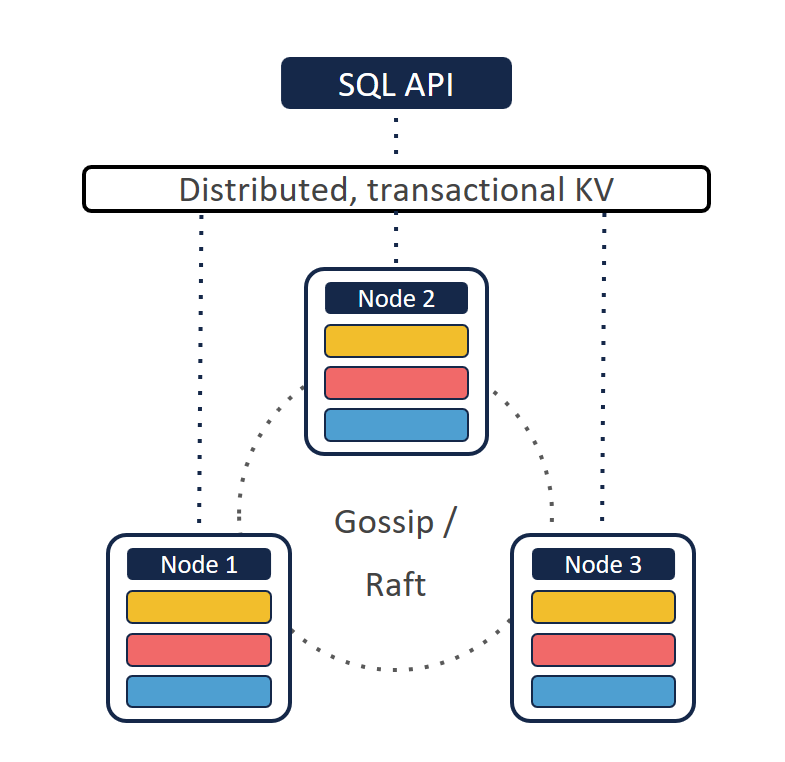
\includegraphics[width=0.5\textwidth]{resources/crdb-arhitecture-overview.png}
\end{center}
\caption{Arhitekturni pregled \cite{CRDB-2017}}
\label{img_crdb_arhitecture_overview}
\end{figure}

\subsubsection{Plasti}
Podatkovna baza CockroachDB je sestavljena iz petih plasti. Plasti med seboj delujejo kot črne škatle. Vsaka plast pa sodeluje le z plastjo direktno nad in pod seboj.

\begin{enumerate}
    \item \textbf{SQL plast:} Prevede SQL poizvedbe v KV operacije.
    \item \textbf{Transakcijska plast:} Omogoča atomične spremembe nad večjim šte\-vi\-lom KV operacij.
    \item \textbf{Porazdelitvena plast:} Predstavi replicirana KV območja kot eno entiteto.
    \item \textbf{Replikacijska plast:} Konsistentno in sinhrono replicira KV obsege v gruči.
    \item \textbf{Shranjevalna plast:} Izvaja bralne in pisalne operacija na disku.
\end{enumerate}

\subsection{SQL plast}

SQL plast predstavlja vmesnik med podatkovno bazo ter ostalimi aplikacijami.  Podatkovna baza CockroachDB implementira velik del SQL standarda \cite{CRDB-sql-standard}. Zunanje aplikacije komunicirajo preko PostgreSQL žičnega protokola. To omogoča enostavno povezavo med zunanjimi aplikacijami in kompatibilnost z obstoječimi gonilniki, orodji ter ORM-ji.

Poleg tega so vsa vozlišča v CockroachDB gruči simetrična, kar pomeni, da se lahko aplikacija poveže na katero koli vozlišče. To vozlišče obdela zahtevek, oziroma ga preusmeri na vozlišče katero zna obdelati zahtevek. To omogoči enostavno porazdelitev bremena.

Ko vozlišče prejme SQL zahtevek, ga najprej razčleni v abstraktno sintaktično drevo. Potem CockroachDB začne s pripravo poizvedovalnega plana. V tem koraku CockroachDB preveri tudi sintaktično pravilnost poizvedb ter nato vse operacije prevedene v KV operacije ter transformira podatke v binarno obliko. S pomočjo poizvedovalnega plana transakcijska plast nato izvede vse operacije.

\begin{table}[H]
\begin{center}
\begin{tabular}{ |l|l| } 
\hline
\textbf{ključ} & \textbf{vrednost} \\
\hline
/system/databases/mydb/id & 51 \\
/system/tables/customer/id & 42 \\ 
/system/desc/51/42/address & 69 \\ 
/system/desc/51/42/url & 66 \\
/51/42/Apple/69 & 1 Infinite Loop, Cupertino, CA \\
/51/42/Apple/66 & http://apple.com/ \\
\hline
\end{tabular}
\end{center}
\caption{Poenostavljen primer preslikave SQL v KV model \cite{CRDB-design}. V podatkovni bazi \texttt{mydb} se nahaja tabela \texttt{customer}, katera ima poleg primarnega ključa še dva stolpca \texttt{address} in \texttt{url}. Zadnja dva zapisa v tabeli predstavljata en vrstico v tabeli \texttt{customer} z primarnim ključem \texttt{Apple}.}
\label{tbl_crdb_sql_kv_mapping}
\end{table}

\subsection{Transakcijska plast}
Podatkovna baza CockroachDB je konsistentna, to dosega tako da, transakcijska plast implementira celotno semantiko ACID transakcij. Vsak stavek predstavlja svojo transakcijo, transakcije pa niso omejene samo na določeno tabelo, obseg ali vozlišče in delujejo preko celotne gruče. To dosežejo z dvofaznim potrditvenim postopkom (angl. two-phase commit):

\begin{enumerate}
    \item \textbf{Faza 1:} Vsaka transakcija najprej kreira transakcijski zapis s statusom v teku (angl. pending). To je podatkovna struktura katera nosi transakcijski ključ in status transakcije. Sočasno, se za pisalne operacije kreira pisalni namen (angl. write intent). Pisalni namen je v osnovi MVCC vrednost označena z zastavico \texttt{<intent>} in kazalcem na transakcijski zapis. Primer MVCC shrambe je prikazan v tabeli \ref{tbl_crdb_mvcc_store}.
    \item \textbf{Faza 2:} V kolikor je transakcijski zapis v status prekinjeno (angl. aborted), se transakcija ponovno izvrši.
    
    Če pa so izpolnjeni vsi pogoji, se transakcija potrdi. Status v transakcijskem zapisu se spremeni v potrjeno (angl. commited). Sočasno se vsem pisalnim namenom povezanim s trenutno transakcijo odstrani zastavico \texttt{<intent>}. 
    \item \textbf{Faza 3 (asinhrono):} Ko se transakcija konča, se vsem potrjenim pisalnim namenom odstrani zastavico \texttt{<intent>} in kazalec na transakcijski zapis. Nepotrjeni pisalni nameni se samo izbrišejo. To se izvede asinhrono, zato vse operacije, preden kreirajo pisalni namen preverijo obstoječi pisalni namen s transakcijskim zapisom in ga ustrezno upoštevajo.
\end{enumerate}

\begin{table}[H]
\begin{center}
\begin{tabular}{ |l|l|l| } 
\hline
\textbf{ključ} & \textbf{čas} & \textbf{vrednost} \\
\hline
A$<$intent$>$ & 500 & nepotrjena vrednost \\
A & 400 & trenutna vrednost \\ 
A & 322 & stara vrednost \\ 
A & 50 & prvotna vrednost \\
B & 100 & vrednost B \\
\hline
\end{tabular}
\end{center}
\caption{Primer MVCC shrambe z pisalnim namenom na ključu A \cite{CRDB-blog-transaction-isolation}.}
\label{tbl_crdb_mvcc_store}
\end{table}

Podatkovna baza CockroachDB privzeto podpira najvišji standardni AN\-SI SQL izolacijski nivo, to je \textit{serializable}. Ta nivo ne dopušča nikakršnih anomalij v podatkih, če obstaja možnost anomalije se transakcija ponovno izvede. Podpira pa tudi zastareli nestandardni izolacijski nivo \textit{snapshot}.

 
\subsection{Porazdelitvena plast}

Vsi podatki v gruči so na voljo preko kateregakoli vozlišča. CockroachDB shranjuje podatke v urejeno vrsto tipa ključ-vrednost. Ta podatkovna stru\-ktu\-ra je namenjena shranjevanju sistemskih kakor tudi uporabniških podatkov. Z nje CockroachDB razbere kje se nahaja podatek in vrednost samega podatka. Podatki so razdeljeni na koščke, katere imenujemo obsegi (angl. ranges). Obsegi so urejeni koščki podatkov preko katerih CockroachDB lahko hitro in učinkovito izvede \textit{lookup} in \textit{scan} operacije.

Lokacija vseh obsegov je shranjena v dvo-nivojskem indeksu. Ta indeks na prvem nivoju sestavlja meta obseg (angl. meta range) imenovan \texttt{meta1}, kateri kaže na meta obseg na drugem nivoju imenovan \texttt{meta2}. Meta obseg \texttt{meta2} pa kaže na podatkovne obsege.

Ko vozlišče prejme zahtevek, v meta obsegih poišče vozlišče katero hrani obseg v najemu (angl. range lease) ter preko tega vozlišča izvede zahtevek. Meta obsegi so predpomnjeni, zato se lahko zgodi, da kažejo na napačno vozlišče. V tem primeru se vrednosti meta obsegov posodobijo.

Privzeto je velikost podatkovnega obsega omejena na 64MiB. To omogoča lažji prenos obsega med vozlišči, poleg tega pa je obseg dovolj velik, da lahko hrani nabor urejenih podatkov, kateri so bolj verjetno dostopani skupaj. Če obseg preseže velikost 64MiB, se razdeli v dva 32MiB podatkovna obsega. Ta dvo-nivojska indeksna struktura omogoča, da naslovimo do \(2^{(18 + 18)} = 2^{36}\) obsegov. Vsak obseg pa privzeto naslavlja \(2^{26}B = 64MiB\) pomnilniške prostora. Teoretično podatkovna baza CockroachDB s privzetimi nastavitvami lahko naslovi do \(2^{(36+26)}B = 4EB\) podatkov. 

\subsection{Replikacijska plast}

Replikacijska plast skrbi za kopiranje podatkov med vozlišči in jih ohranja v konsistentnem stanju. To doseže preko soglasnega algoritma (angl. consensus algorithm) Raft. Ta algoritem zagotovi, da se večina vozlišč v gruči strinja z vsako spremembo v podatkovni bazi. S tem, kljub odpovedi posameznega vozlišča, ohrani podatke v konsistentnem stanju poleg tega pa zagotovi nemoteno delovanje podatkovne baze (visoko razpoložljivost).

Število vozlišč, ki lahko odpove brez, da bi s tem vplivalo na delovanje podatkovne baze je enako:
\[(r - 1)/2 = f \text{, če}\ r = 3, 5, 7, ...\ \text{in}\ r <= N\]
Kjer je \(N\) število vseh vozlišč v gruči, \(r\) faktor replikacije liho število večje ali enako tri in manjše ali enako številu vseh vozlišč v gruči. Ter \(f\) maksimalno število vozlišč, ki še lahko odpove brez, da bi vplivalo na delovanje podatkovne baze. Na primer če je replikacijski faktor \(r = 3\), gruča lahko tolerira odpoved enega vozlišča \(f = 1\).

Za vsak obseg obstaja Raft skupina, kjer je eno vozlišče, ki vsebuje repliko, označena kot "vodja". Vodja je izvoljen in koordinira vse pisalne zahtevke za določen obseg. V idealnih pogojih je vodja Raft skupine tudi najemnik obsega (angl. leaseholder).


\subsection{Shranjevalna plast}

CockroachDB za shranjevanje uporablja KV shrambo RocksDB. RocksDB zagotavlja atomične skupine pisalnih zahtevkov, kar CockroachDB potrebuje za zagotavljanje transakcij. RocksDB preko kompresije ključev zagotavlja učinkovito shrambo podatkov.

CockroachDB uporablja MVCC pristop in hrani več verzij vsakega podatka. Podatkovna baza CockroachDB preko MVCC pristopa omogoča poizvedbe v zgodovino \texttt{SELECT...AS OF SYSTEM TIME}. Privzeto stare verzije podatka pretečejo po 24 urah in so počiščene s shrambe.

\section{Lastnosti}
Razvoj podatkovne baze CockroachDB je bil usmerjen prvotno v funkcionalnosti in še le kasneje v optimizacije. Tako verzija 1.0.0 omogoča razvijalcem večina potrebnih funkcionalnosti, verzija 2.0.0 pa je poleg manjših funkcionalnosti prinesla predvsem optimizacije.

\subsection{Enostavnost}
Podatkovna baza CockroachDB strmi k enostavnosti upravljanja in vzdr\-že\-van\-ja. Večina kompleksnosti je skrite končnemu uporabniku. Izogiba se zunanjim odvisnostim in je na voljo kot ena sama binarna datoteka. Minimalno za zagon gruče je potrebno na vsakem vozlišču zagotoviti sinhronizacije ure, priporočena je uporaba zunanje Google NTP storitve ter namestiti CockroachDB binarno datoteko na vsako vozlišče in jo zagnati.

\subsection{Uporabniški vmesnik in nadzorovanje}
Poleg podatkovne baze CockroachDB vsebuje tudi spletni administratorski vmesnik, ki je prikazan na sliki \ref{img_crdb_admin_ui}. Administratorski vmesniki nudi vizualizacije raznih časovnih metrik o delovanju posameznih vozlišč, kakor tudi celotne gruče. Omogoča pregled dnevnikov in pripomore k lažjemu odkrivanju težav v gruči. CockroachDB omogoča tudi izvoz metrik v odprtokodno rešitev Prometheus, katera nam omogoča shrambo, obdelavo, vizualizacije in obveščanje nad časovnimi vrstami.

\begin{figure}[H]
\begin{center}
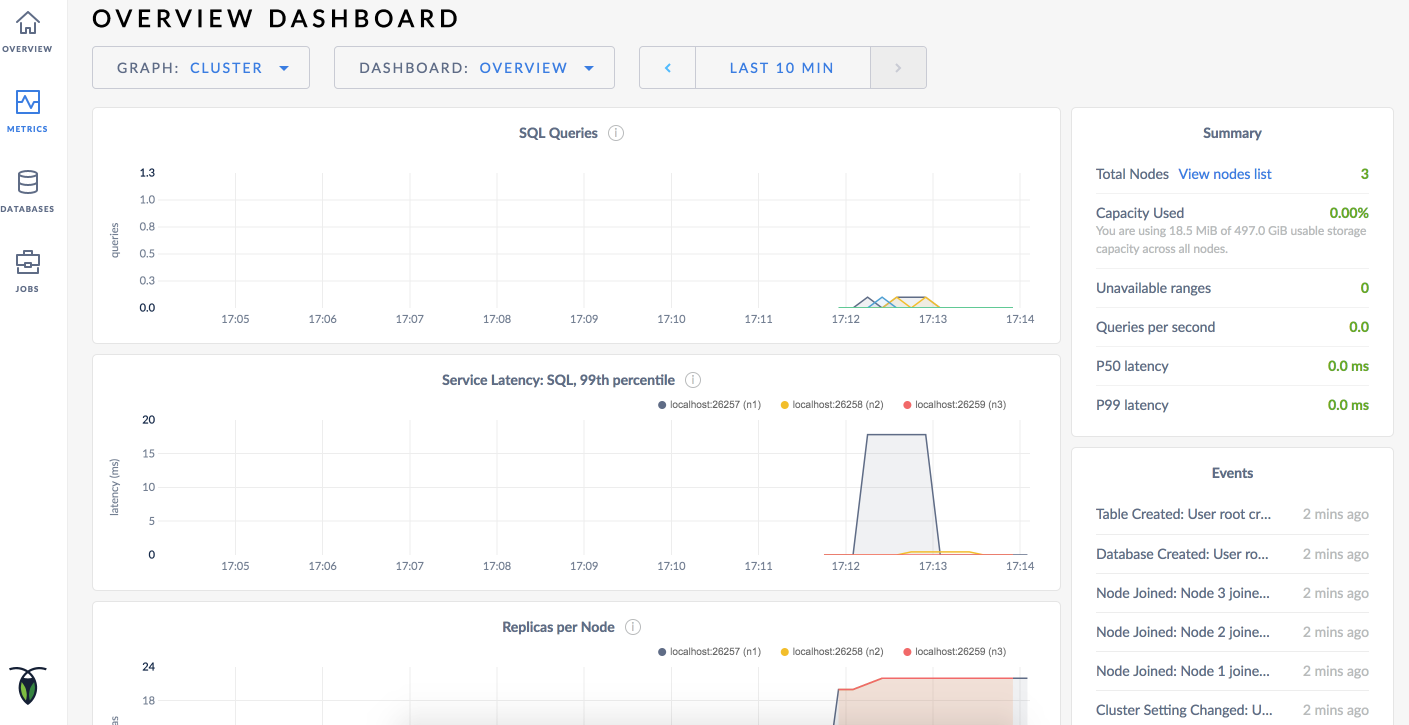
\includegraphics[width=1\textwidth]{resources/crdb_admin_ui.png}
\end{center}
\caption{Primer spletnega administratorski vmesnika.}
\label{img_crdb_admin_ui}
\end{figure}

\subsection{SQL}
CockroachDB, kakor večina relacijskih podatkovnih baz, podpira podmnožico SQL standarda \cite{CRDB-sql-standard}. Poleg tega implementira nekatere najpogostejše raz\-ši\-rit\-ve, razširitve specifične za PostgreSQL ter svoje razširitve. V spodnjih podpoglavjih bom v grobem opisal, kaj od jezika SQL ponuja CockroachDB, bolj podroben opis pa se nahaja v uradni dokumentaciji \cite{CRDB-sql-features}.

\subsubsection{Podatkovni tipi}
CockroachDB podpira podatkovne tipe kot so \texttt{ARRAY}, \texttt{BOOL}, \texttt{BOOL}, \texttt{BYTES}, \texttt{COLLATE} (podobno kot \texttt{STRING} vendar upošteva specifike jezika), \texttt{DATE}, \texttt{DE\-CI\-MAL}, \texttt{FLOAT}, \texttt{INET} (IPv4 in IPv6 naslovi), \texttt{INTERVAL} (časovni interval), \texttt{JSONB}, \texttt{SERIAL} (\texttt{INT} z avtomatsko kreirano številko, priporočena uporaba \texttt{UUID}), \texttt{STRING}, \texttt{TIME}, \texttt{TIMESTAMP} in \texttt{UUID}. CockroachDB ne podpira podatkovnih tipov \texttt{XML}, \texttt{UNSIGNED INT} ter \texttt{SET} in \texttt{ENUM}.

\subsubsection{Shema}
CockroachDB podpira vse standardne ukaze za kreiranje, spreminjanje in odstranjevanje tabel, stolpcev, omejitev in indeksov. Od podatkovnih omejitev podpira vse standardne, to so: \texttt{NOT NULL}, \texttt{UNIQUE}, \texttt{CHECK}, \texttt{FOREIGN KEY} in \texttt{DEFAULT}. Izjema je \texttt{PRIMARY KEY}, to omejitev lahko nastavimo samo ob kreiranju tabele in je kasneje ne moremo spreminjati. Če omejitve \texttt{PRIMARY KEY} ne nastavimo v času kreiranja tabele, CockroachDB v ozadju sam kreira skriti stolpec z tipom \texttt{UUID}, saj je ta pomemben za samo delovanje podatkovne baze.

Poizvedovanje sheme je na voljo na standardni način, preko virtualne sheme \texttt{informationq\_schema}.

Prožilci še niso podprti in tudi ne načrtovani za naslednje verzije.

\subsubsection{Transakcije}
CockroachDB podpira ACID transakcije, katere so lahko distribuirane preko celotne gruče. Privzeto transakcije uporabljajo najvišji izolacijski nivo \texttt{SE\-RI\-AL\-IZ\-ABLE}, omogoča pa še zastareli izolacijski nivo \texttt{SNAP\-SHOT}. Ostali standardni izolacijski nivoji niso podprti.

\subsubsection{Tabelarični izrazi}
CockroachDB podpira referenciranje tabel, pogledov, poizvedb, tabelaričnih funkcij. Od \texttt{JOIN} operacij omogoča \texttt{INNER}, \texttt{LEFT}, \texttt{RIGHT}, \texttt{FULL}, \texttt{CROSS}, vendar pa te operacije še niso optimizirane. Da bi dosegli optimalno delovanje je potrebno \texttt{JOIN} operacije pravilno omejiti.

\subsubsection{Operatorji, skalarni izrazi, logični izrazi in funkcije}
CockroachDB implementira večji del standardnih operatorjev, skalarnih izrazov, logičnih izrazov ter funkcij. Slabo podporo zagotavlja konsturktu \texttt{EXISTS} in skalarnim pod-poizvedbam. Podpira poizvedovanje po tipu JSON, omogoča iskanje z POSIX regularnimi izrazi ter implementira okenske funkcije (funkcije katere se izvedejo nad podmnožico, tipično ob uporabi \texttt{GROUP BY}).

Uporabniške funkcije niso podprte in tudi ne načrtovane za naslednje verzije. Shranjene procedure so načrtovane za eno od naslednjih verzij.

\subsection{Poslovna licenca}

CockroachDB je odprtokodna in zastonjska podatkovna baza. Večina potrebnih funkcionalnosti omogoča zastonjska različica, poleg tega pa ponuja tudi poslovno licenco. Poslovna licenca omogoča strankam:

\begin{itemize}
    \item svetovanje,
    \item tehnično pomoč,
    \item geografsko distribucijo na nivoju ene vrstice,
    \item vizualizacijo geografsko distribuirane gruče na zemljevidu,
    \item nadzor dostopa na nivoju skupin in
    \item distribuirano kreiranje in obnova varnostnih kopij.
\end{itemize}

\subsection{Podprta orodja, gonilniki in ORM-ji in skupnost}

Podatkovna baza CockroachDB implementira standardni SQL \cite{CRDB-sql-standard}, za komunikacijo med odjemalcem in strežnikom pa uporablja PostgreSQL žični protokol, kar omogoča dobro kompatibilnost z obstoječimi PostgreSQL komponentami.

Na uradni spletni dokumentaciji je za jezike Go, Java, .NET, C++, NodeJS, PHP, Python, Ruby, Rust, Clojure ter Elixir objavljen seznam podprtih gonilnikov in ORM-jev. Za te CockroachLabs v času pisanja zagotavlja le beta podporo \cite{CRDB-meta-drivers-orms}.

Od orodij za upravljanje z podatkovno bazo nam CockroachLabs ponuja konzolno aplikacijo \texttt{cockroach sql}. Od grafičnih orodij nudijo beta podporo za pgweb, dbglass, Postico, PSequel, TablePlus in Valentina studio \cite{CRDB-meta-vizualizers}. Orodje pgweb ima trenutno najbolj zdravo in aktivno skupnost, je odprtokodno in podpira vse glavne operacijske sisteme (Windows, OSX in Linux). Aplikacijo dostopamo preko spletnega brskalnika in podpira funkcionalnosti kot so:

\begin{itemize}
    \item pregled podatkovne baze in sheme
    \item izvedba in analiza SQL poizvedb
    \item zgodovina poizvedb
    \item izvoz podatkov v formatu CSV, JSON in XML
\end{itemize}

Izvirna koda podatkovne baze CockroachDB je javno dostopna preko GitHub repozitorija \texttt{cockroachdb/cockraoch} \cite{cockroachdb/cockroach}. Projekt ima zdravo skupnost, kateremu trenutno sledi približno 14 tisoč navdušencev. Poleg GitHub repozitorija, kjer se odvija ves razvoj, vodenje nalog in pomoč, CockroachLabs vodi še spletno stran \cite{CRDB-home} (dokumentacija, form, blog, mediji), Gitter kanal \cite{CRDB-gitter} in Docker repozitorij \cite{CRDB-docker}.

\chapter{Primerjalna analiza zmogljivosti CockroachDB}

Primerjalna analiza zmogljivosti (angl. performance benchmarking) je postopek za primerjavo enega sistema z ostalimi podobnimi sistemi. V mojem primeru bom z orodjem YCSB primerjal podatkovni bazi CockroachDB ter PostgreSQL z nameščeno razširitvijo Citus (v nadaljevanju samo Citus). 

Za primerjavo z Citus sem se odločil zaradi lažje izvedbe ter bolj primerljivih rezultatov. Obe podatkovni bazi CockroachDB in Citus sta po nekaterih lastnostih zelo podobni. Obe podatkovni bazi implementirat standardni SQL ter komunicirata preko PostgreSQL žičnega protokola. 

Za orodje YCSB sem se odločil, saj podpira vmesnik JDBC, katerega podpirata tudi obe podatkovni bazi poleg tega pa je enostaven za uporabo. Orodje YCSB sem bolj podrobno opisal v poglavju \ref{YCSB_about}. Ob iskanju najprimernejšega orodja sem pregledal naslednja orodja:

\begin{itemize}
    \item \textbf{TPC:}\\ TPC (angl. transaction processing performance council) \cite{TPC-home} je ne profitna organizacija, katera nudi preverljive podatke TPC zmogljivostnih analiz podatkovnih baz. TPC definira več različnih standardnih testov, kateri simulirajo različne realne obremenitve. Te testi so točno opisani in strogo omejeni. Najbolj poznan tip testa za transakcijske obremenitve je TPC-C, za analitične pa TPC-H.

    To so standardizirani testi in bi bili najbolj primerni, vendar pa so zelo kompleksni. Uradnih TPC testov za podatkovno bazo CockroachDB še ne obstaja.
    \item \textbf{pgbench:}\\ Je enostavno orodje namenjeno PostgreSQL podatkovni bazi. Simulira ne standardno TPC-C obremenitev.
    
    Orodje pgbench v času izvajanja testov še ni bilo kompatibilno z podatkovno bazo CockroachDB.
    \item \textbf{cockroachdb/loadgen:}\\ Je orodje namenjeno CockroachDB podatkovni bazi. Orodje vsebuje nabor testov kot so TPC-C, TPC-H in YCSB. Te orodja interno uporabljajo za zmogljivostno primerjavo med verzijami CockroachDB podatkovne baze. Kasneje je bil objavljena tudi objava na njihovem blogu, kjer so primerjali rezultate TPC-C obremenitve med podatkovnima bazama CockroachDB in Amazon Aurora.

    Orodje je enostavno, vendar ne omogoča zmogljivostne analize PostgreSQL podatkovne baze.
    \item \textbf{Apache JMeter:}\\ Je orodje primarno namenjeno izvajanju obremenitvenih testov. Tega orodje omogoča izvajanje obremenitvenih testov preko JDBC vmesnika.
    
    Orodje je zelo konfigurabilno vendar pa ne omogoča v naprej definiranih obremenitvenih testov in je težko za uporabo.
    \item \textbf{YCSB:}\\ YCSB (angl. Yahoo! Cloud Serving Benchmark) je orodje namenjeno za primerjavo zmogljivostnih metrik med raznimi podatkovnimi bazami.
\end{itemize}

V naslednjih podpoglavjih bom opisal točen postopek s katerim sem izvedel primerjalno analizo. Opisal bom arhitekturo, pripravo posameznih konfiguracij, pripravo podatkov in samo testiranje. Na koncu bom predstavil rezultate zmogljivostne analize ter ugotovitve.

\section{Hipoteze}
Pred začetkom izvajanja primerjalne analize sem postavil naslednje hipoteze:
\begin{enumerate}
    \item CockroachDB bo na enem vozlišču nekoliko počasnejši od PostgreSQL podatkovne baze.
    \iffalse
    Razlog za to hipotezo je, da je CockroachDB na trgu dobro leto in še ni dokončno optimizirana. Medtem, ko je PostgreSQL na trgu dobrih 20 let.
    \fi
    \item CockroachDB bo zaradi linearne skalabilnosti na treh vozliščih skoraj tri krat bolj zmogljiv.
\end{enumerate}

\section{Arhitektura}
Testno okolje sestavljajo štiri vozlišča označena z \texttt{n0}, \texttt{n1}, \texttt{n2} in \texttt{n3}. Specifikacije strojne opreme so opisane v tabeli \ref{tbl_benchmarking_nodes_hw}. Vsa vozlišča imajo nameščen Ubuntu 16.04 LTS, Docker 18.03.0-ce ter ntpd, ki je konfiguriran glede na produkcijska priporočila  CockroachDB podatkovne baze \cite{CRDB-ntpd-configuration}.

Vozlišča so med seboj povezana preko gigabitnega Ethernet omrežja v Docker Swarm \cite{Docker-Swarm-Mode} gručo. Vozlišče \texttt{n0} je v vlogi vodje, vozlišča \texttt{n1}, \texttt{n2} in \texttt{n3} pa so v vlogi delavcev. Za uporabo Docker Swarm tehnologije sem se odločil zaradi enostavnosti postavitve okolja ter lažje ponovljivosti testov.

\begin{table}[H]
\begin{center}
\begin{tabular}{ |l|l|l|l|l| } 
\hline
 & \textbf{procesor} & \textbf{pomnilnik} & \textbf{trdi disk} \\
\hline
n0 & Intel Core2 Quad CPU Q9400 & 4GB & SAMSUNG HD753LJ \\
n1 & Intel Core i5 CPU 650 & 4GB & WDC WD10EARS-22Y5B1 \\ 
n2 & Intel Core i7-3770 & 8GB & ST500DM002-1BD142 \\ 
n3 & Intel Core i5-2400 & 4GB & Hitachi HDS721050CLA662 \\
\hline
\end{tabular}
\end{center}
\caption{Specifikacije strojne opreme, katere se razlikujejo med posameznimi vozlišči.}
\label{tbl_benchmarking_nodes_hw}
\end{table}

\subsection{Odjemalec}
Vozlišče n0 je v vlogi odjemalca. Na njem teče program, ki zažene podatkovno bazo, obnovi podatke, izvaja teste in beleži rezultate. Podroben opis delovanja odjemalca se nahaja v poglavju \ref{YCSB_benchmarking_steps}.

\subsection{Strežnik}
V vlogi strežnika so vozlišča \texttt{n1}, \texttt{n2} in \texttt{n3}. Na njih teče ali CockroachDB ali PostgreSQL z nameščeno razširitvijo Citus. V primeru, da gre za konfiguracijo z enim vozliščem, podatkovna baza teče na vozlišču \texttt{n2}.

\section{Citus}
\label{benchmarking/citus}
\hl{TODO}

\section{YCSB}
\label{YCSB_about}
YCSB \cite{brianfrankcooper/YCSB} je razširljiva in odprtokodna rešitev za primerjalno analizo zmogljivosti. Največkrat se uporablja za zmogljivostno analizo različnih NoSQL podatkovnih baz. Podpira veliko število različnih podatkovnih baz kot so  Mongo, Couchbase, S3, Redis, itd. Poleg tega pa podpira tudi JDBC vmesnik, preko katerega sem primerjal CockroachDB ter PostgreSQL podatkovni bazi. YCSB nudi šest enostavnih predefiniranih tipov obremenitev \cite{YCSB-core-workloads} označenih z A, B, C, D, E in F.

\section{Testiranja YCSB obremenitev}
\label{YCSB_benchmarking_steps}
Testiranje je potekalo iz odjemalca, torej vozlišča \texttt{n0}. Meritev je bilo veliko, zato sem pripravil program s katerim sem si pomagal. Program je enostaven in ni prenosljiv. Izvorna koda in rezultati meritev so na voljo na GitHub repozitoriju \cite{matjazmav/diploma-ycsb}. V tem poglavju bom opisal vse korake kateri so bili potrebni za izvedbo meritev.

\subsection{Namestitev programske opreme}
Na vozlišču \texttt{n0} sem namestil naslednjo programsko opremo:
\begin{itemize}
    \item YCSB (verzija 0.12.0) \cite{brianfrankcooper/YCSB} je orodje namenjeno za izvedbo zmogljivostne analize ter primerjavo med različnimi podatkovnimi bazami. Samo orodje sem bolj natančno opisal v poglavju \ref{YCSB_about}.
    \item Ansible (verzija 2.5.0) \cite{Ansible} je orodje za avtomatizacijo, uporabil sem ga zaradi lažjega konfiguriranja gruče preko SSH povezave.
    \item Go (verzija 1.10.1) \cite{Golang} je programski jezik, v katerem je napisan program za avtomatizacijo testiranja. Za programski jezik Go sem se odločil, zaradi njegove enostavnosti.
\end{itemize} 

\subsection{Priprava podatkov}
\label{benchmarking-prepare-data}
Program za avtomatizacijo predpostavlja, da imajo vsa vozlišča na točno določeni lokaciji pripravljene podatke za obnovo fizične podatkovne baze. Pred vsakim testom se podatki kopirajo v začasno mapo, nad katero kasneje baza izvaja operacije. Po končanem testu se začasna mapa izbriše.

V spodnjih korakih je opisan postopek, po katerem sem za vsako bazo ter za vsako konfiguracijo (eno vozlišče in tri vozlišča) pripravil podatke. Vse konfiguracijske datoteke, ki so uporabljene v spodnjih primerih so na voljo na GitHub repozitoriju \texttt{matjazmav/diploma-ycsb} \cite{matjazmav/diploma-ycsb}.

\subsubsection{Citus}
\begin{enumerate}
    \item Z Docker Swarm konfiguracijsko skripto (\texttt{stacks/postgres-n1.yml}) sem pognal Citus podatkovno bazo na vozlišču \texttt{n2}.
    \item Na vozlišču \texttt{n2} sem ročno kreiral shemo katero potrebuje YCSB za svoje delovanje.
    \begin{listing}[H]
    \begin{minted}{vim}
        CREATE DATABASE ycsb;
        \c ycsb;
        CREATE TABLE usertable (
            YCSB_KEY VARCHAR(255) PRIMARY KEY,
            FIELD0 TEXT, FIELD1 TEXT,
            FIELD2 TEXT, FIELD3 TEXT,
            FIELD4 TEXT, FIELD5 TEXT,
            FIELD6 TEXT, FIELD7 TEXT,
            FIELD8 TEXT, FIELD9 TEXT
        );
    \end{minted}
    \label{code-ycsb-schema-postgres}
    \end{listing}
    \item Nato sem generiral podatke. V bazo na vozlišču \texttt{n2} sem z YCSB orodjem naložil 5 milijonov zapisov, kar na disku zasede približno 6GB prostora.
    \begin{listing}[H]
    \begin{minted}{vim}
        ycsb load jdbc \
            -P workloads/workloada \
            -P configs/postgres-n1.properties \
            -p threadcount=16 \
            -p recordcount=5000000
    \end{minted}
    \label{code-ycsb-load-postgres}
    \end{listing}
    \item Podatkovno bazo sem varno ustavil ter naredil varnostno kopijo fizične podatkovne baze na disku.
    \item Nato sem Docker Swarm konfiguracijsko skripto (\texttt{stacks/\\postgres-n3.yml}) pognal Citus podatkovno bazo na treh vozliščih.
    \item Na vozliščih \texttt{n1} in \texttt{n3} sem kreiral shemo definirano v točki 2.
    \item Nato sem na vozlišču \texttt{n2} povezal še vozlišči \texttt{n1} ter \texttt{n3} in kreiral distribuirano tabelo. Podatki v tabeli \texttt{usertable} so se enakomerno porazdelili med vsa tri vozlišča.
    \begin{listing}[H]
    \begin{minted}{vim}
        \c ycsb;
        SELECT * FROM master_add_node('<n1 ip addr>', 5432);
        SELECT * FROM master_add_node('<n2 ip addr>', 5432);
        SELECT create_distributed_table('usertable', 'ycsb_key');
    \end{minted}
    \label{code-ycsb-add-node-citus}
    \end{listing}
    \item Po končani konfiguraciji sem bazo varno ustavil ter naredil varnostno kopijo podatkov na disku.
\end{enumerate}

\subsubsection{CockroachDB}
\begin{enumerate}
    \item Z Docker Swarm konfiguracijsko skripto (\texttt{stacks/\\cockroachdb-n1.yml}) sem pognal CockroachDB bazo na vozlišču \texttt{n2}.
    \item Na vozlišču \texttt{n2} sem ročno kreiral shemo katero potrebuje YCSB za svoje delovanje.
    \begin{listing}[H]
    \begin{minted}{vim}
        CREATE DATABASE ycsb;
        USE ycsb;
        CREATE TABLE usertable (
            YCSB_KEY VARCHAR(255) PRIMARY KEY,
            FIELD0 TEXT, FIELD1 TEXT,
            FIELD2 TEXT, FIELD3 TEXT,
            FIELD4 TEXT, FIELD5 TEXT,
            FIELD6 TEXT, FIELD7 TEXT,
            FIELD8 TEXT, FIELD9 TEXT
        );
    \end{minted}
    \label{code-ycsb-schema-cockroach}
    \end{listing}
    \item Nato sem generiral podatke. V bazo na vozlišču \texttt{n2} sem z YCSB orodjem naložil 5 milijonov zapisov, kar na disku zasede približno 6GB prostora.
    \begin{listing}[H]
    \begin{minted}{vim}
        ycsb load jdbc \
            -P workloads/workloada \
            -P configs/cockroachdb-n1.properties \
            -p threadcount=16 \
            -p recordcount=5000000
    \end{minted}
    \label{code-ycsb-load-cockroach}
    \end{listing}
    \item Podatkovno bazo sem varno ustavil ter naredil varnostno kopijo fizične podatkovne baze na disku.
    \item Nato sem Docker Swarm konfiguracijsko skripto (\texttt{stacks/\\cockroachdb-n3.yml}) pognal CockroachDB bazo na treh vozliščih.
    \item Baza je sama zaznala dve novi vozlišči in pričela avtomatsko z replikacijo podatkov na ostala dva vozlišča. Ko se je replikacija končala sem bazo varno ustavil ter naredil varnostno kopijo fizične podatkovne baze na disku.
\end{enumerate}


\subsection{Program za avtomatizacijo}
Vozlišče \texttt{n0} je v vlogi odjemalca. Na njem teče program, ki za vse kombinacije parametrov (baza, število vozlišč, število sočasnih povezav) izvaja teste in beleži rezultate. Program predpostavlja, da obstajajo za vsako konfiguracijo v naprej pripravljeni podatki na točno določenem mestu. Postopek za pripravo podatkov sem opisal v poglavju \ref{benchmarking-prepare-data}. Program v grobem za vsako kombinacijo parametrov izvede naslednje koraka:
\begin{enumerate}
    \item Obnovi vnaprej definirane podatke (\texttt{cp -a})
    \item Zažene podatkovno bazo (\texttt{docker stack up})
    \item Izvede YCSB test (\texttt{ycsb run jdbc ...})
    \item Zabeleži rezultat v datoteko CSV
    \item Ustavi podatkovno bazo (\texttt{docker stack rm})
    \item Počisti podatke (\texttt{rm -rf})
\end{enumerate}

Koraki 2, 3, 4 in 5 se ponovijo za vsak tip obremenitve v točno določenem vrstnem redu (A, B, C, F, D). Vrstni red obremenitev je pomemben \cite{YCSB-core-workloads}, ker obremenitve tipa A, B, C in F ne vstavljajo novih zapisov. Obremenitev tipa D pa vstavlja nove zapise, zato je po vsaki izvedbi potrebno obnoviti bazo na prvotno stanje.

Zaradi morebitnih odstopanj sem vse teste ponovil trikrat.

\section{Testiranje stičnih operacij}
\hl{TODO}

\section{Rezultati}
Vsi rezultati so na voljo na GitHub repozitoriju \texttt{matjazmav/diploma-ycsb} \cite{matjazmav/diploma-ycsb}. V mapi \texttt{results} se nahajajo datoteke z neobdelani podatki. Analizo rezultatov pa sem izvedel v excel datoteki \texttt{results.xlsx}. Po analizi sem prišel do spodnjih rezultatov.

\newpage

\begin{figure}[H]
    \begin{center}
    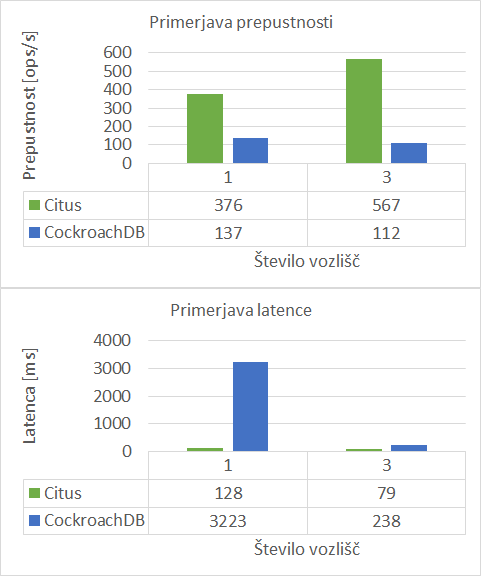
\includegraphics[width=1\textwidth]{resources/top-level-comparison.png}
    \end{center}
    \caption{Groba primerjava povprečne prepustnosti in latence med obema podatkovnima bazama na enem in treh vozliščih.}
    \label{img_ycsb_results_top_level_comparison}
    \end{figure}

\newpage

\begin{figure}[H]
\begin{center}
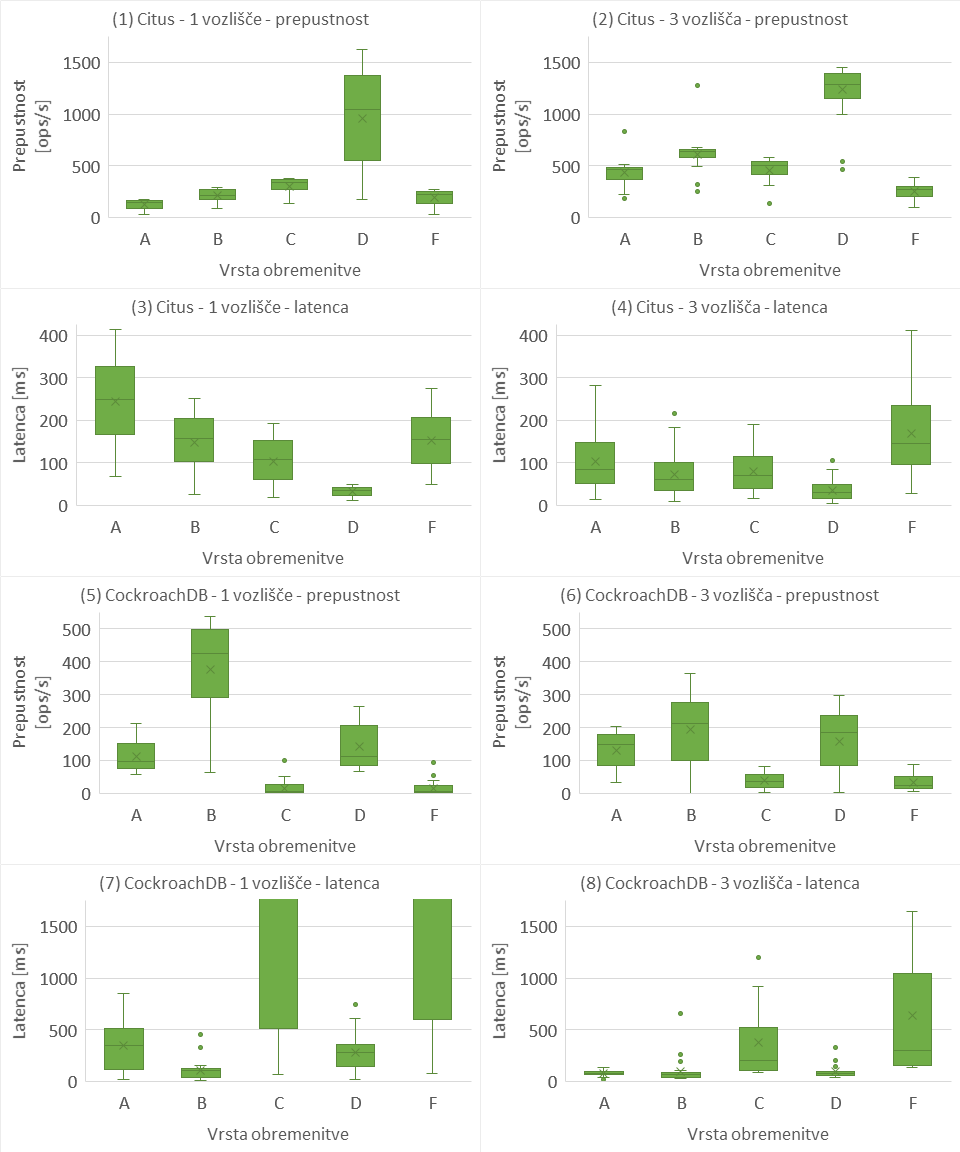
\includegraphics[width=1\textwidth]{resources/comparison-throughputnlatency-bnw.png}
\end{center}
\caption{Prikazuje primerjavo prepustnosti in latenc glede na vrsto obremenitve med podatkovno bazo Citus in CockroachDB. Graf \textbf{CockroachDB - 1 vozlišče - latenca [ms]} je zaradi lažje primerjave odrezan.}
\label{img_ycsb_results_bnw_comparison}
\end{figure}

\newpage

\begin{figure}[H]
\begin{center}
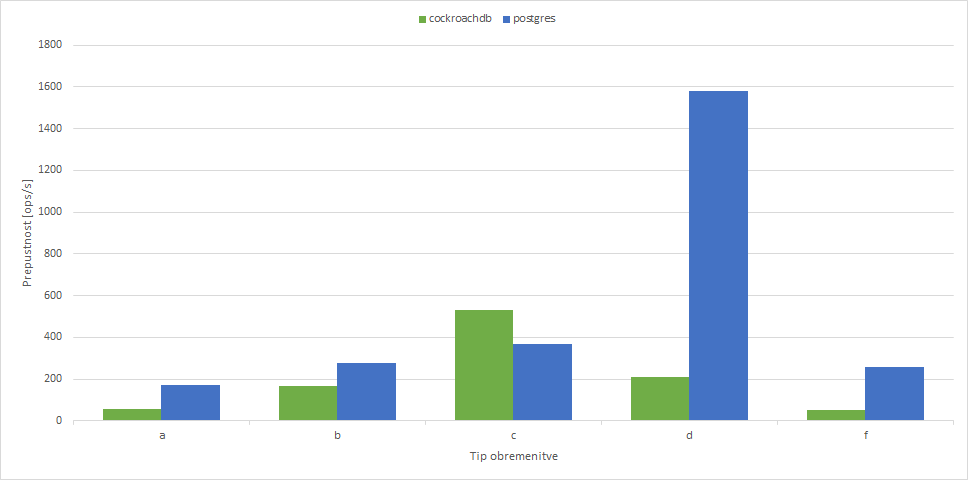
\includegraphics[width=1\textwidth]{resources/maxThroughput-n1-v2.png}
\end{center}
\caption{Primerjava maksimalne prepustnosti glede na tip obremenitve pri enem vozliščih.}
\label{img_ycsb_results_max_throughput_n1}
\end{figure}

\begin{figure}[H]
\begin{center}
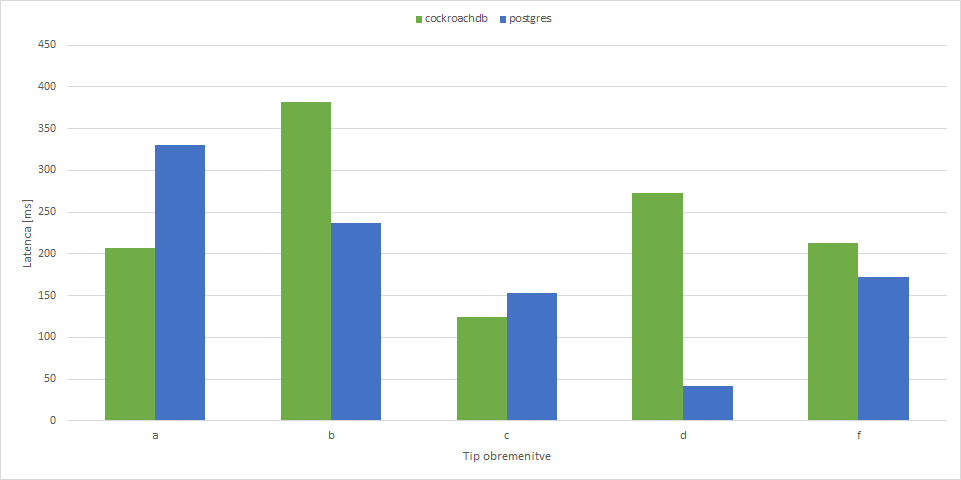
\includegraphics[width=1\textwidth]{resources/maxThroughput-latency-n1-v2.png}
\end{center}
\caption{Latenca pri maksimalni obremenitvi glede na tip obremenitve pri enem vozliščih.}
\label{img_ycsb_results_max_throughput_latency_n1}
\end{figure}

\newpage

\begin{figure}[H]
\begin{center}
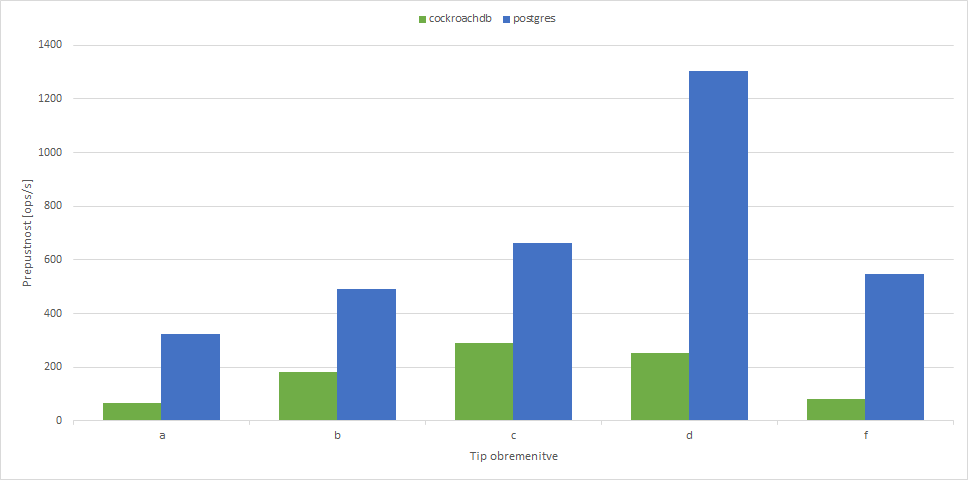
\includegraphics[width=1\textwidth]{resources/maxThroughput-n3-v2.png}
\end{center}
\caption{Primerjava maksimalne prepustnosti glede na tip obremenitve pri treh vozliščih.}
\label{img_ycsb_results_max_throughput_n3}
\end{figure}

\begin{figure}[H]
\begin{center}
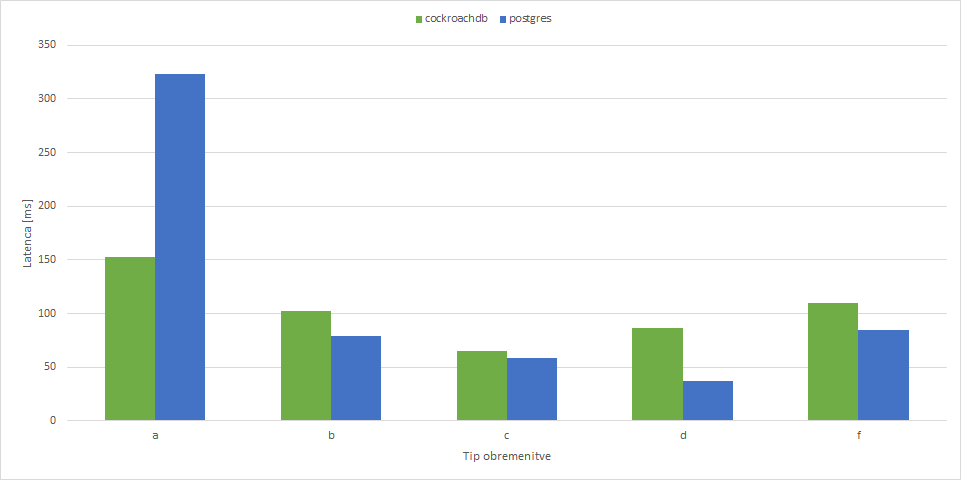
\includegraphics[width=1\textwidth]{resources/maxThroughput-latency-n3-v2.png}
\end{center}
\caption{Latenca pri maksimalni obremenitvi glede na tip obremenitve pri treh vozliščih.}
\label{img_ycsb_results_max_throughput_latency_n3}
\end{figure}

\section{Ugotovitve}
Zmogljivostna analiza je pokazala, da se podatkovna baza Citus pri večini obremenitev, katere sem testiral, odziva bitveno bolje kot podatkovna baza CockroachDB.

S slike \ref{img_ycsb_results_top_level_comparison} je razvidno, da CockroachDB v primerjavi s Citus dosega 2,7 krat manjšo prepustnost na enem vozlišču in kar 5 krat manjšo prepustnost na treh vozliščih. Pri primerjavi latence pa je CockroachDB v primerjavi s Citus na enem vozlišču dosegel približno 25,2 krat večjo latenco, na treh vozljiščih pa samo še 3 krat večjo.

S slike \ref{img_ycsb_results_bnw_comparison} je razvidno, da je podatkovna baza CockroachDB v primerjavi s podatkovno bazo Citus manj stabilna. To se odraža na posameznih grafih saj so podatki pri podatkovni bazi CockroachDB veliko bolj razpršeni.

% Izjema je bila latenca pri vrsti obremenitve A, ker je CockroachDB dosegel približno pol manjšo latenco. Kljub temu pa je bila prepustnost bistveno nižja.

% Druga izjema se je pojavila pri obremenitvi tipa C na enem vozlišču, kjer je CockroachDB dosegel približno eno četrtino večjo prepustnost kot PostgreSQL.

\subsection{Hipoteza 1}
\textit{CockroachDB bo na enem vozlišču nekoliko počasnejši od PostgreSQL podatkovne baze.}

\ \\
Razlog za to hipotezo je, da je podatkovna baza PostgreSQL že dolgo na trgu \cite{Postgres-first-release} in je uporabljena na mnogih projektih. Zato je zmogljivostno bolje optimizirana kakor CockroachDB. CockroachDB pa je na trgu od leta 2015. Prvo stabilno verzijo (1.0.0) so objavili maja 2017 \cite{CRDB-2017}, druga verzija (2.0.0) pa je bila objavljena aprila 2018. Vsaka verzija je dodala veliko novih funkcionalnosti.

% \begin{figure}[H]
% \begin{center}
% 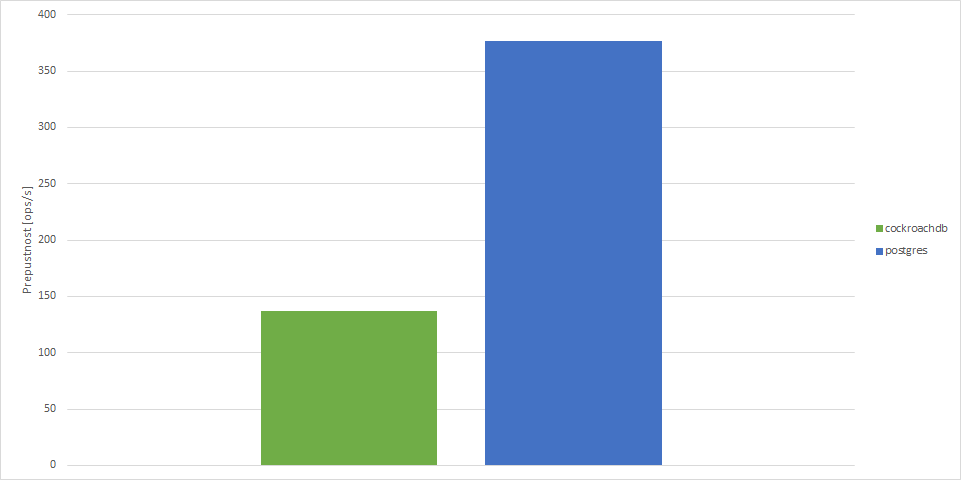
\includegraphics[width=1\textwidth]{resources/throughput-comparison-n1-v2.png}
% \end{center}
% \caption{Primerjava povprečne prepustnosti na enem vozlišču.}
% \label{img_ycsb_results_throughptu_comparison_n1}
% \end{figure}

Hipotezo sem potrdil, kar je razvidno tudi na sliki \ref{img_ycsb_results_top_level_comparison}. Podatkovna baza CockroachDB v primerjavi z PostgreSQL dosega približno 2,7 krat nižjo prepustnost.

Podobno zmogljivostno primerjavo so decembra 2017 izvedli na zasebni raziskovalni univerzi v Bruslju \cite{CRDB-2017}. Z orodjem YCSB (verzija 0.12.0) so primerjali obremenitve tipa A, B in C. Ugotovili so, da se podatkovna baza CockroachDB (verzija 1.1.3) v primerjavi z PostgreSQL (verzija 9.6.5) odziva približno 10 krat slabše kakor PostgreSQL. V njihovem primeru so testno okolje postavili v Amazon oblaku, vsako bazo na treh vozljiščih.

\subsection{Hipoteza 2}
\textit{CockroachDB bo zaradi linearne skalabilnosti na treh vozliščih skoraj tri krat bolj zmogljiv.}

\ \\
Vsa vozlišča povezana v CockroachDB gručo so simetrična, kar pomeni, da vsa vozlišča opravljajo enake naloge. Ob predpostavki, da se uporabniki enakomerno razporedijo preko vseh vozlišč, ter, da je obremenitev enakomerna, naj bi bila rast prepustnosti linearna \cite{CRDB-design}.

% \begin{figure}[H]
% \begin{center}
% 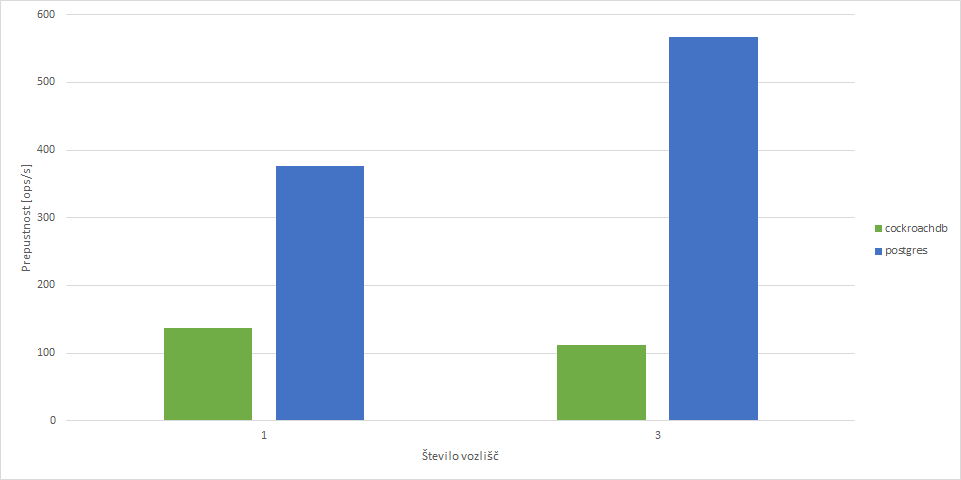
\includegraphics[width=1\textwidth]{resources/scaling-throughput-v2.png}
% \end{center}
% \caption{Primerjava povprečne prepustnosti ob skaliranju baze na tri vozlišča.}
% \label{img_ycsb_results_scaling_throughptu_comparison}
% \end{figure}

To hipotezo sem ovrgel. Meritve so pokazale, da podatkovna baza CockroachDB doseže celo slabšo prepustnost na treh vozliščih. To razvidno na sliki \ref{img_ycsb_results_top_level_comparison}.

Razlog za tak rezultat naj bi bila primerjava med konfiguracijo na enem in treh vozliščih \cite{CRDB-YCSB-perf-analisis}. CockroachDB na treh vozliščih s privzetimi nastavitvami začne z postopkom replikacije podatkov. Privzeto je vsak podatek repliciran trikrat, enkrat na vsakem vozlišču. CockroachDB tako zagotavlja konsistenco in visoko razpoložljivost.

Rezultati neuradne TPC-C zmogljivostne analize, katero so izvedli v Co\-ckroachLabs, kažejo, da je CockroachDB linearno skalabilen \cite{CRDB-TPCC-perforamance-report}. Ob skali\-ranju z 3 na 30 vozlišč ter ob sorazmernem povečanju obremenitve so dosegli tudi sorazmerno večjo prepustnost.

Prišel sem do ugotovitve, da je CockroachDB linearno skalabilna podatkovna baza, (1) če je obremenitev enakomerno porazdeljena med vsa vozlišča in (2) faktor replikacije ob skaliranju ostane konstanten.

Na podlagi teh ugotovitev sem pripravil optimistično oceno rasti povprečne prepustnosti. Obe bazi se v idealnih pogojih in do neke mere skalirata linearno, kar je prikazano na sliki \ref{img_ycsb_results_scaling_throughptu_prediction}. Vendar pa se pri PostgreSQL konfiguraciji vsi odjemalci direktno povezujejo na eno vozlišče (koordinatorja), to vozlišče je ozko grlo (točka A), saj bo ob večanjem v neki točki prišlo do zasičenosti resursov \cite{Citus-add-coordinator}. V neki točki (točka B) pa bo CockroachDB presegel prepustnost podatkovne baze Citus.

\begin{figure}[H]
\begin{center}
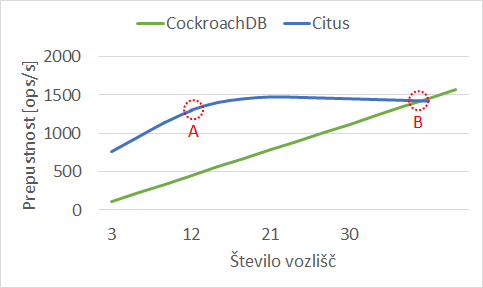
\includegraphics[width=1\textwidth]{resources/scaling-throughput-prediction-v2.png}
\end{center}
\caption{Optimistična ocena rasti povprečne prepustnosti. Pri podatkovni bazi Citus, se v točki A linearna rast konča. V točki B pa je ima CockroachDB že večjo prepustnost. Graf je le simboličen in ne predstavlja realnih meritev.}
\label{img_ycsb_results_scaling_throughptu_prediction}
\end{figure}


\chapter{Sklepne ugotovitve}

V diplomskem delu smo pregledali lastnosti  ter najpogosteje uporabljene mehanizme in pristope pri implementacijah novih arhitektur NewSQL podatkovnih baz. Opisali smo arhitekturo in lastnosti izbrane NewSQL podatkovne baze CockroachDB \cite{CRDB-home}. Podatkovno bazo CockroachDB smo kasneje praktično testirali. Izvedeli smo primerjalno analizo zmogljivosti med podatkovno bazo CockroachDB in PostgreSQL \cite{postgres} (z nameščeno razširitvijo Citus \cite{citus}). Veliko časa smo vložili v postavitev testnega okolja in bili pozorni, da smo odpravili čim več spremenljivk, ki bi lahko vplivale na testne scenarije. Testno okolje je bilo sestavljeno s štirih starejših računalnikov, kateri so bili povezani preko gigabitnega omrežja, na njih pa je tekel Ubuntu Server \cite{ubuntu-server} in Docker \cite{docker}. Testno okolje smo v začetku nadzirali preko Telegraf agenta \cite{telegraf}, InfluxDB podatkovne baze za shranjevanje časovnih podatkov \cite{influxdb} in Grafane za vizualizacijo podatkov \cite{grafana}. Kljub trudu, ki smo ga vložili v postavitev testnega okolja, bi le tega lahko še izboljšali. Za boljšo primerljivost zmogljivostnih metrik, bi morala imeti vsa vozlišča enako strojno opremo, testirati pa bi moral še konfiguracije z več kot tremi vozlišči. Izvedbo testiranja smo avtomatizirali. Z orodjem YCSB \cite{brianfrankcooper/YCSB} smo izvajali različne zmogljivostne teste, rezultate pa shranjevali v CSV datoteko in jih kasneje analizirali.

Primerjalna analiza zmogljivosti je pokazala, da je podatkovna baza Cock\-roachDB kljub enostavnim obremenitvam, katere vrši orodje YCSB, v večini primerov bistveno slabša od PostgreSQL podatkovne baze. V povprečju je imela podatkovna baza Cock\-roachDB 3 krat večjo latenco in 5 krat manjšo prepustnost kakor podatkovna baza PostgreSQL na treh vozljiščih.
% Poleg tega pa je z večanjem sočasnih povezav zmogljivost padala bistveno hitreje kot pri podatkovni bazi PostgreSQL.
Kljub slabšim rezultatom zmogljivostne analize, se moramo zavedati, da je težko pošteno primerjati dve zelo različni podatkovni bazi. Podatkovna baza PostgreSQL je bistveno starejša in zato bolj stabilna ter optimizirana. CockroachDB pa je na trgu šele dobri dve leti in je trenutno še vedno bolj funkcionalno usmerjena. Za smiselno odločitev pri izbiri podatkovne baze moramo poleg zmogljivostnih metrik upoštevati tudi druge, kot so poizvedovalni jezik, podpora transakcijam, zrelost sistema, skupnost, zmogljivost, težavnost postavitve ter vzdrževanja, ostale lastnosti specifične za vsako podatkovno bazo, ...

Podatkovna baza CockroachDB ima močno in aktivno skupnost. Na spletu najdemo že kar nekaj vrednotenj drugih avtorjev, od raznih primerjalnih analiz \cite{kaur2017performance, Benchmarking-GCS-CRDB-NuoDB, CRDB-tpcc-vs-aurora, CRDB-2017}, do Jepsen testov konsistence in obnašanja sistema med napakami \cite{CRDB-jepsen, CRDB-jepsen-diy}.

Kljub temu, da je CockroachDB relativno nova podatkovna baza, jo podjeta že uporabljajo. Na primer podjetje Baidu \cite{crdb-baidu}, uporablja CockroachDB pri dveh novih aplikacijah, ki sta predhodno uporabljale MySQL podatkovno bazo. Ti dve aplikaciji obsegata približno 2TB podatkov in ustvarita približno 50M zapisov na dan. Podjetje Kindred \cite{crdb-kindred}, ki se ukvarja z spletnim igralništvom. Z letom 2014 pa so začeli s prehodom na globalni trg. Imajo kompleksen ekosistem z več kot 200 mikrostoritev. Ta arhitektura omogoča elastičnost vendar pa mora biti skoraj v celoti avtonomna. CockroachLabs poizkuša s podjetji sodelovati, nekatera podjetja so tudi prispevala del funkcionalnosti. Podjetja katera so se odločila za uporabo podatkovne baze CockroachDB, ciljajo globalni trg, poleg tega pa želijo poenostaviti postavitev in vzdrževanje, tako v oblak, kako tudi na svoji infrastrukturi.

Glede na znanje katerega smo pridobil skozi diplomsko delo, menimo, da je podatkovna baza CockroachDB primerna za nove transakcijsko usmerjene (OLTP) aplikacije, katere zahtevajo konsistenco in visko razpoložljivost hkrati pa ciljajo hitrorastoč globalni trg. Za aplikacije kjer je čas do trga zelo pomemben in kjer si ne moremo privoščiti velikih stroškov vzdrževanja. Pred odločitvijo moramo oceniti še podprto sintakso SQL jezika \cite{CRDB-sql-features} in morebitne ostale lastnosti \cite{CRDB-limitations}. Podatkovna baza CockroachDB trenutno ni primerna za scenarije kateri zahtevajo kompleksne stične operacije, nizko latenco in aplikacije katere so analitično usmerjene (OLAP) \cite{CRDB-FAQ}.

V prihodnje bi bilo zanimivo raziskati in primerjati še zelo podobno in prav tako odprtokodno podatkovno bazo TiDB \cite{PingCAP-home}. TiDB je trenutno še zelo mlad produkt, z verzijo 1.0.0, ki je izšla sredi oktobra 2017 in verzijo 2.0.0 iz aprila 2018. TiDB prav tako idejno temelji na podatkovni bazi Google Spanner in se v nekaterih arhitekturnih lastnostih zelo ujema s podatkovno bazo CockroachDB. Najbolj očitna razlika je, da je arhitektura ločena na tri večje komponente, poleg tega za sinhronizacijo ure uporablja drugačen pristop. Razvijalci podatkovne baze TiDB obljubljajo, da je podatkovna baza primerna za hibridne transakcijske in analitične obremenitve.

Zanimivo bi bilo tudi razširiti zmogljivostno primerjalno analizo izvedeno v tej diplomski nalogi. Distribuirane podatkovne baze kot je CockroachDB so primerne za okolja z vsaj tremi vozlišči, zanimivo bi bilo ugotoviti kaj se dogaja, ko v gručo povežemo še več vozlišč. Poleg osnovnih YCSB obremenitev, bi bilo zanimivo preveriti še druge, kot sta TCP-C in TCP-H. V tej diplomski nalogi smo se tem obremenitvam izognil, saj orodje \cite{cockroachdb/loadgen} še ni bilo podprto za primerjavo s podatkovno bazo PostgreSQL.


\newpage %dodaj po potrebi, da bo številka strani za Literaturo v Kazalu pravilna!
\ \\
\clearpage
\addcontentsline{toc}{chapter}{Literatura}
\bibliographystyle{plain}
\bibliography{bibliography}


\end{document}

